\documentclass[10pt, oneside, ngerman]{article}


\author{Philipp Jetzlaff}
\title{Projektdokumentation}

%%%%%%%%%%%%%%%%% P A C K A G E S %%%%%%%%%%%%%%%%%%%%%%%%%%%%%%%%%%%%%%%%%%%%%%%%%%%%%
%Package to create a custom header, that is printed on every page in the document.
\usepackage{fancyhdr}
%Package to include graphics.
\usepackage{graphicx}
\usepackage{helvet}
%Package to defines the paper enviroment
\usepackage[a4paper, headheight=60pt, bottom=20mm, left=25mm, right=25mm]{geometry}
%Package to defines hyperrefs in the document. E.g references to figures or tables
\usepackage{hyperref}
\usepackage{nameref}
%Packages to use sourcecode in this document
\usepackage{listings}
\usepackage{caption}
%Packages for table
\usepackage{tabularx}
\usepackage{multirow}
\usepackage{tablefootnote}

%Package to use colors in the documents. For example \rowcolor
\usepackage{color, colortbl}
\usepackage{babel}
\usepackage{microtype}
\usepackage{pdfpages}


%Define Header
\fancyhf{}
\fancyhead[R]{
\includegraphics[width=0.11\textwidth]{OktoPOS.png}}
\fancyhead[L]{
  \uppercase{Erweiterung eines Onlineserivce}\\
  \vspace{1pt}
  \small{Anbindung der OktoPOS Cash Software an den internen Übersetzungsdienst}\\ 
  \vspace{4pt}
  \scriptsize{\leftmark}
}
\fancyfoot[L]{Philipp Jetzlaff}
\fancyfoot[R]{\thepage}
\renewcommand{\headrulewidth}{1pt}
\renewcommand{\footrulewidth}{1pt}
%Define Colors
\definecolor{LightCyan}{rgb}{0.88,1,1}
\definecolor{blue-green}{rgb}{0.0, 0.87, 0.87}
\definecolor{carolinablue}{rgb}{0.6, 0.73, 0.89}
\definecolor{lightgray}{rgb}{0.83, 0.83, 0.83}
%Define Codeblockfont
%Define imagepath
\graphicspath{{src/img/}}
%Define Listings apperiance
\lstset{basicstyle=\ttfamily}
%Overwrite naming for list
\renewcommand{\listfigurename}{Abbildungsverzeichnis}
\renewcommand{\listtablename}{Tabellenverzeichnis}
\renewcommand{\contentsname}{Inhaltsverzeichnis}
%\renewcommand{\lstlistlistingname}{Listingsverzeichnis}
\renewcommand{\tablename}{Tabelle}
\renewcommand{\figurename}{Abbildung}
% Create new commands for work with refs.
\newcommand{\tabsecref}[1]{\hyperref[{#1}]{Tabelle \thesubsection. \nameref*{#1}}}
\newcommand{\figsecref}[1]{\hyperref[{#1}]{Abbildung \thesubsection. \nameref*{#1}}}
\newcommand{\attsecref}[1]{\hyperref[{#1}]{Anhang \thesubsection. \nameref*{#1}}}
\newcommand{\secref}[1]{\hyperref[{#1}]{\nameref{#1}}}
\newcommand{\tabref}[1]{\nameref{#1}}
\renewcommand{\familydefault}{\sfdefault}

\begin{document}
\sloppypar
%Define Header and footer
  \pagestyle{fancy}
  
  %Deckblatt einfügen
  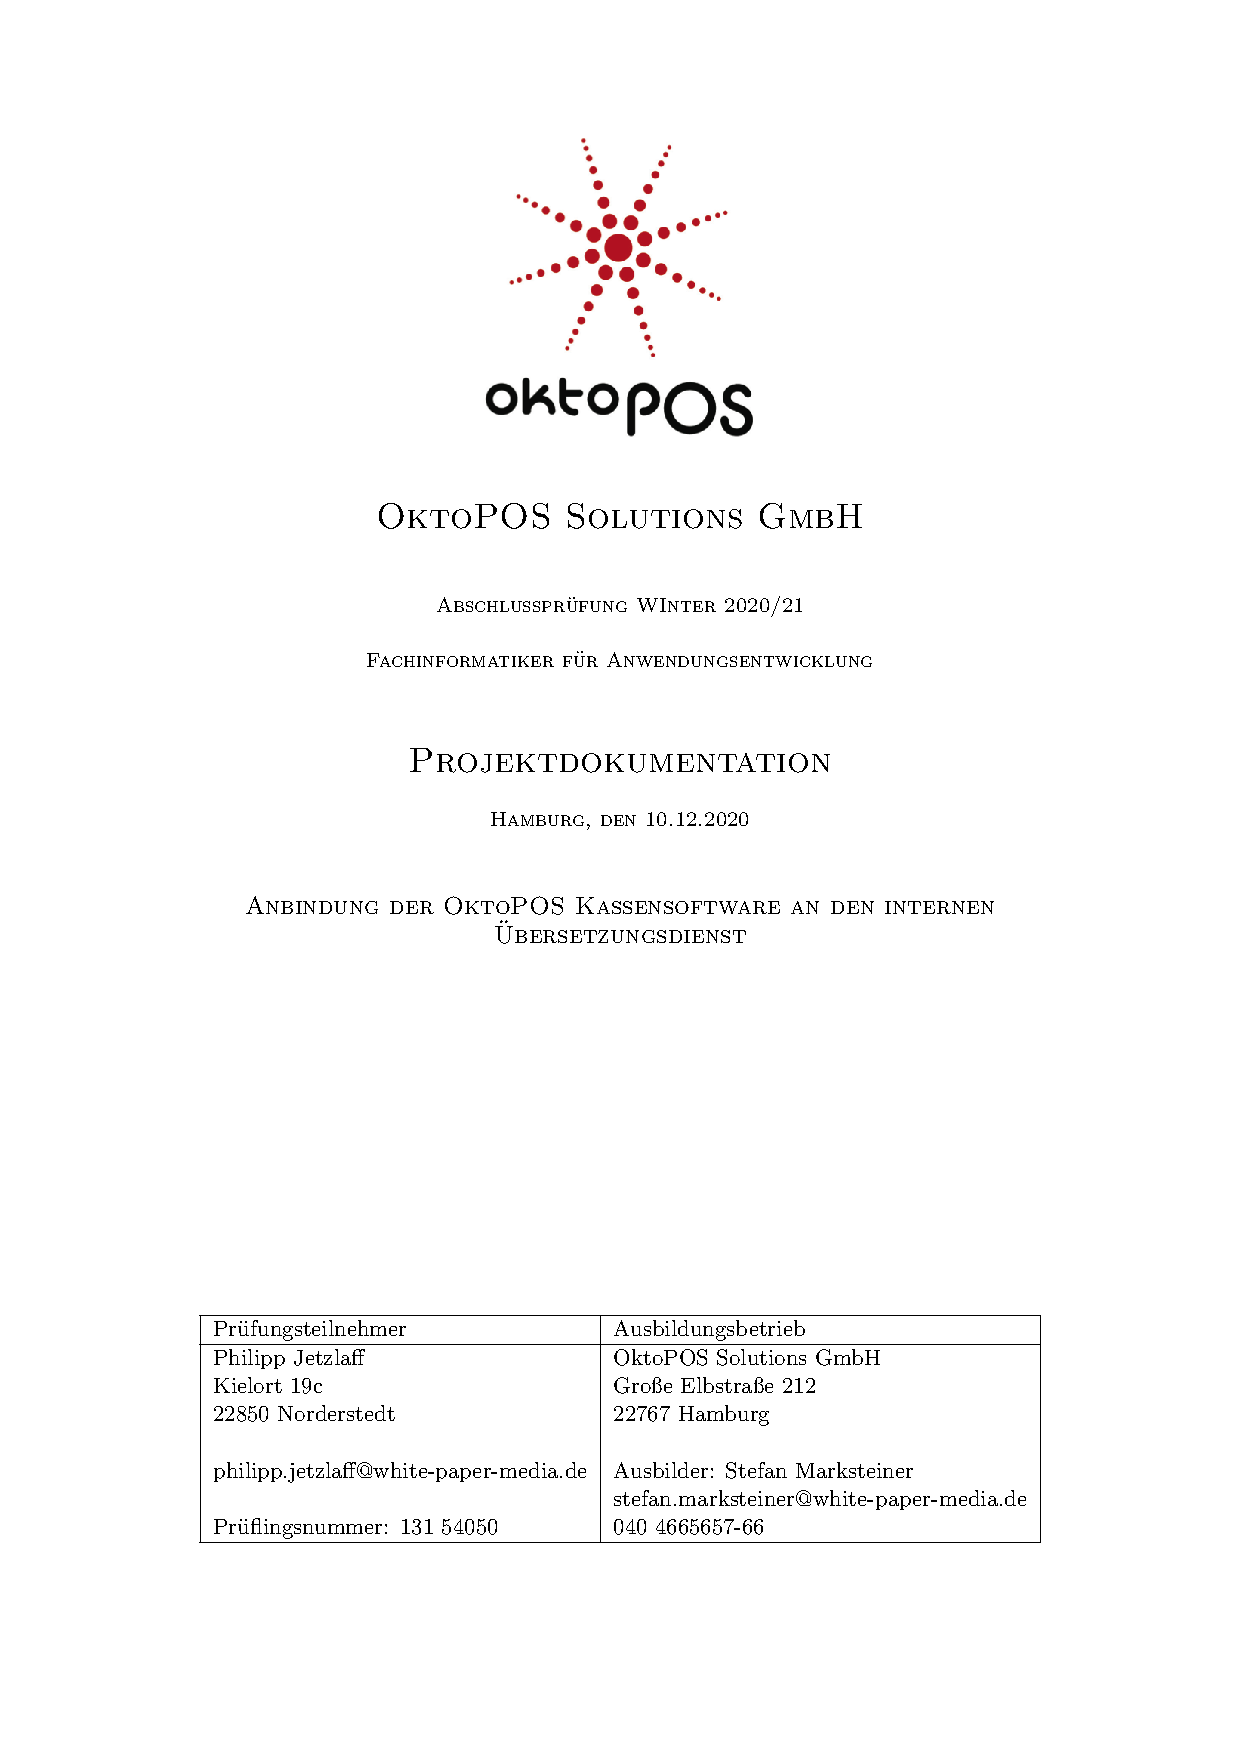
\includepdf{cover/cover.pdf}
  %table of contents
  \pagenumbering{roman}
  \tableofcontents
  \newpage
  \addcontentsline{toc}{section}{\listfigurename}
  \listoffigures
  \addcontentsline{toc}{section}{\listtablename}
  \listoftables
  \lstlistoflistings
  \newpage
  \section{Glossar}
  \begin{tabular}{p{0.25\textwidth} l}
    \textbf{Begriff} & \textbf{Definition}\\
    & \\
    Annotations & Markierungen im Quellcode für die ORM Konfiguration. \\
    & \\
    Buildserver & Server für die kontinuierliche Integration von Software.\\
    & \\
    Caching & Zwischenspeichern von Daten.\\
    & \\
    Classpath & Verzeichnis in dem die Java-Class-Dateien liegen.\\
    & \\
    Client & In der Client-Server-Architektur entspricht der Client einem Nutzer. \\
    & \\
    Dashboard & Übersicht.\\
    & \\
    Datenbankschema & Aufbau der Relationen in einer Relationalen Datenbank.\\
    & \\
    Deployment & Ausliefern von Software.\\
    & \\
    DDL & Befehle zur Definition von Tabellen und anderer Datenstrukturen.\\
    & \\
    \multirow{2}{*}{Dependency Injection} & Entwurfsmuster, welches die Abhängigkeiten eine\\ & Objekts zur Laufzeit reglementiert.\\
    & \\
    DML & Befehle zur Datenmanipulation und Datenabfrage.\\
    & \\
    \multirow{2}{*}{Entität} & Ein eindeutig bestimmbares Objekt, über das die Datenbank \\ & Informationen speichern soll.\\
    & \\
    \multirow{2}{*}{HashMap} & Eine Datenstruktur in der Informatik um Werte einem \\ & eindeutigen Key zugewiesen werden können.\\
    & \\
    Interface & Schnittstellen, entweder für weitere Programme oder Benutzer.\\
    & \\
    JSON & JavaScript Object Notation.\\
    & \\
    Langauagelevel & Die Version einer Programmiersprache.\\
    & \\
    Multilingualität & Die Verwendung von mehreren Sprachen.\\
    & \\
    \multirow{2}{*}{ORM} & Objektrelation-Mapping. Eine Technik in der Softwareentwicklung\\ & um Objekte in Entitäten umzuwandeln.\\
    & \\
    POS-System & Point-Of-Sales.\\
    & \\
    Property-key & Schlüssel zur Identifizierung eines Wertes innerhalb einer Datei.\\
    & \\
    \multirow{2}{*}{Property-Pair} & Kombination aus einem Property-Key und \\ & einer Property-Value. Z.B. foo=bar.\\
    & \\
    Property-Value & Wert, welcher einem Schlüssel in einer Datei zugewiesen ist.\\
    & \\
  \end{tabular}
  \begin{tabular}{p{0.25\textwidth} l}
    \textbf{Begriff} & \textbf{Definition}\\
    & \\
    \multirow{2}{*}{Stylesheet} & Dokument um den Style von Klassen innerhalb eines \\ &HTML Dokuments zu beschreiben.\\
    & \\
    Token  & Platzhalter.\\
    & \\
    \multirow{2}{*}{Webservice} & Stellt eine Schnittstelle für die Kommunikation \\ & über Rechnernetze zur Verfügung.\\
  \end{tabular}
  \newpage
  \pagenumbering{arabic}
  \section{Einleitung}
    Im Rahmen der IHK-Abschlussprüfung für den Ausbildungsberuf Fachinformatiker für Anwendungsentwicklung
    wurde diese Projektdokumentation angefertigt. Sie dokumentiert den Ablauf und die Herangehensweise 
    welche zur Lösung der, im Vorfeld von dem zuständigen Ausbilder definierten, Projektanforderungen beigetragen haben. 
    Der Ausbildungsbetrieb OktoPOS Solutions GmbH ist ein mittelständisches Unternehmen mit Hauptsitz in Hamburg. Hauptdienstleistung der
    OktoPOS Solutions GmbH sind das POS-System OktoPOS Cash und das Personalmanagementsystem OktoCareer.
    %Interdisplinare Berührungspunkte
  \subsection{Projektbeschreibung}\label{sec:projectdesc}
    Das von der OktoPOS Solutions entwickelte Produkt OktoPOS Cash ist ein, im internationalen Raum, genutztes POS System. 
    Für eine anwenderfreundliche Nutzung ist die gesamte Textausgabe des Front-End in diversen Sprachen verfügbar. 
    Zur Realisierung der multilingualen Textausgabe werden für die angezeigten Texte Platzhalten (Tokens) im Kassencode verwendet. 
    Die anzuzeigenden Texte in den jeweiligen Sprachen werden als Schlüssel-Werte-Paar in den Übersetzungsdateien hinterlegt, 
    wobei der im Kassencode verwendete Token als Schlüssel verwendet wird. 
    Für jede unterstützte Sprache gibt es genau eine Übersetzungsdatei.
    Die Erweiter- und Wartbarkeit der Übersetzungsdateien sind nach aktuellem Stand stark optimierungsbedürftig. 
    Es gibt keine Garantie dafür, dass jede Datei dieselbe Anzahl an Tokens beinhaltet bzw. es gibt keinen direkten Überblick 
    über den Übersetzungsstand der Dateien. 
    Es kann vorkommen, dass die Übersetzungen von unternehmensfremden Personal angefertigt, 
    die mit der Struktur solcher Dateien nicht vertraut sind. Dadurch verlängert sich die Einarbeitungszeit der Übersetzer und kostet 
    nicht notwendige Ressourcen.\\ %EVENTUELL SATZ
    Neben der unwirtschaftlichen Nutzung von Ressourcen, ist der Stand der Übersetzung innerhalb des Kassensystems abhängigkeit von der Releaseversion der Kassensoftware. 
    Übersetzungs- sowie Rechtschreibfehler in den Übersetzungen können erst nach Release einer neuen Kassenversion behoben werden.\\
    In der Abteilung für das Personalmanagementsystem OktoCareer wird nach einem ähnlichen Prinzip die Mulitlingualität des Front-Ends unterstützt. Dabei 
    werden allerdings die genutzten Tokens über den unternehmensinternen Übersetzungsdienst TranslationService abgebildet und in einem benutzerfreundlichen Front-End übersetzt und verwaltet.
    Mit der Anbindung der Kassensoftware an den unternehmensinternen Übersetzungsdienst TranslationService sollen die oben genannten Schwächen im Übersetzungsworkflow 
    und dem Management der Übersetzungsdateien behoben werden. 
    Außerdem soll über ein zusätzlichen Dienst der aktuellste Stand an Übersetzungen im Livebetrieb zur Verfügung gestellt werden können.
  \subsection{Projektziel}
    Ziel des Projektes ist es, durch die Anbindung der Kassensoftware an den unternehmensinternen TranslationService,
    den Prozess der Übersetzung von dem Releaseprozess zu entkoppeln und Versionsupdates der Übersetzungsdateien im Livebetrieb zu ermöglichen.
    Im Rahmen des Projektes soll die Integrität des Kassencodes erhalten bleiben. Daher ist es notwendig den Updateprozess der Übersetzungsdateien
    in einen externen Dienst auszulagern.\\
    Der Transaltionservice ist zu so zu erweitern, dass Tokens und Übersetzungen in Abhängigkeit zu ihrer Version empfangen bzw. bereitgestellt werden können.
    Nach aktuellem Stand, ist der TranslationService nicht in der Lage, Tokens und Übersetzungen zu versionieren. 
    Das Anlegen einer neuen Version erfolgt von außen über eine zu schaffende Schnittstelle. Im Front-End des TranslationService, soll die Möglichkeit gegeben 
    werden, die Tokens und den Stand der Übersetzung in Abhängigkeit zu ihrer Version anzeigen zu lassen.\\
    Ziel ist es durch eine Versionierung der Tokens und Transaltions eine Kassenversion kompatible Version der Übersetzungsdateien zu exportieren. Dabei können die Anzahl der Tokens, sowie die 
    mögliche Übersetzung einer Textstelle in Versionen unterscheiden.\\
    Da das Erstellen der Schnittstellen, die Implementierung der neuen Anwendung und das Testen der Komponenten die veranschlagten 70 Stunden in Anspruch nehmen,
    werden das Deployment der Minianwendung sowie die Anpassung des Deploymentprozesses der Kassensoftware an eine andere Abteilung ausgelagert, die in der Kostenaufstellung mit aufgenommen werden. %IN DIE KOSTENAUFSTELLUNG
  \subsection{Projektumfeld}\label{sec:projectEnv}
    Das Projekt ist ein Auftrag der Entwicklungsabteilung der Kassensoftware OktoPOS Cash. Das Java gestützte POS System nutzt Übersetzungsdateien um Textstellen im Front-End in verschiedenen Sprachen darzustellen.
    Während der Entwicklung an der Kassesoftware, speziell beim Implementieren von Features, werden in machen Fällen neue Übersetzungstokens eingeführt. Der Entwickler muss dabei den Token in jede einzelne Datei schreiben. 
    Die Übersetzer der Abteilung OktoCareer nutzen den TranslationService für die Übersetzungen an ihrem Personalmanagementsystem. 
    Der TranslationSerivce bietet die Datenstruktur, welche mit geringen Aufwand erweitert werden kann um die neuen Anforderungen zu erfüllen. 
  \subsection{Projektabgrenzung}
    Die grundlegende Struktur des TranslationService ist bereits implementiert und wird produktiv im Unternehmen genutzt. Das Projekt beschränkt sich hinsichtlich der Arbeiten an dem Transaltionservice nur auf das Hinzufügen der 
    neuen Schnittstellen, dem Erweitern der Datenbank und den daraus resultierenden Änderungen der vorhandenen Entitäten und Anpassungen im Front-End.
    Die beschränkte Dauer, die für dieses Projekt zur Verfügung gestellt wurde, hat zur Folge, dass Teile zur Realisierung des Gesamtprojektes an andere Abteilungen ausgelagert werden mussten.
    Dazu gehört neben dem GitWebhook, welcher die Übersetzungsdateien der Kasse an den Übersetzungsdienst übergibt, auch das Deployment des neuen Dienstes.
  \section{Projektplanung}
  \subsection{Entwicklungsprozess}\label{sec:dev:prc}
    Im Vorfeld der Planung wurde von dem Autor ein Entwicklungsprozess festgelegt. Der Entwicklungsprozess legt fest, in welcher Reihenfolge 
    die notwendigen Projektphase geplant und bearbeitet werden können.
    Der Autor hat sich in Absprache mit den Projektleitern der betreffenden Projekte auf das erweiterte Wasserfallmodell geeinigt.\\
    Ergänzend zu den iterativen Aspekten des Wasserfallmodells erlaubt das erweiterte Wasserfallmodell einen schrittweisen Rückgang zu vorhergehenden Phasen,
    sofern in der aktuellen Phase ein Fehler aufgetreten ist.\\
    Die Abbildung \ref{abb:vg} zeigt das genutzte Wasserfallmodell. 
    \begin{figure}[ht]
      \centering
      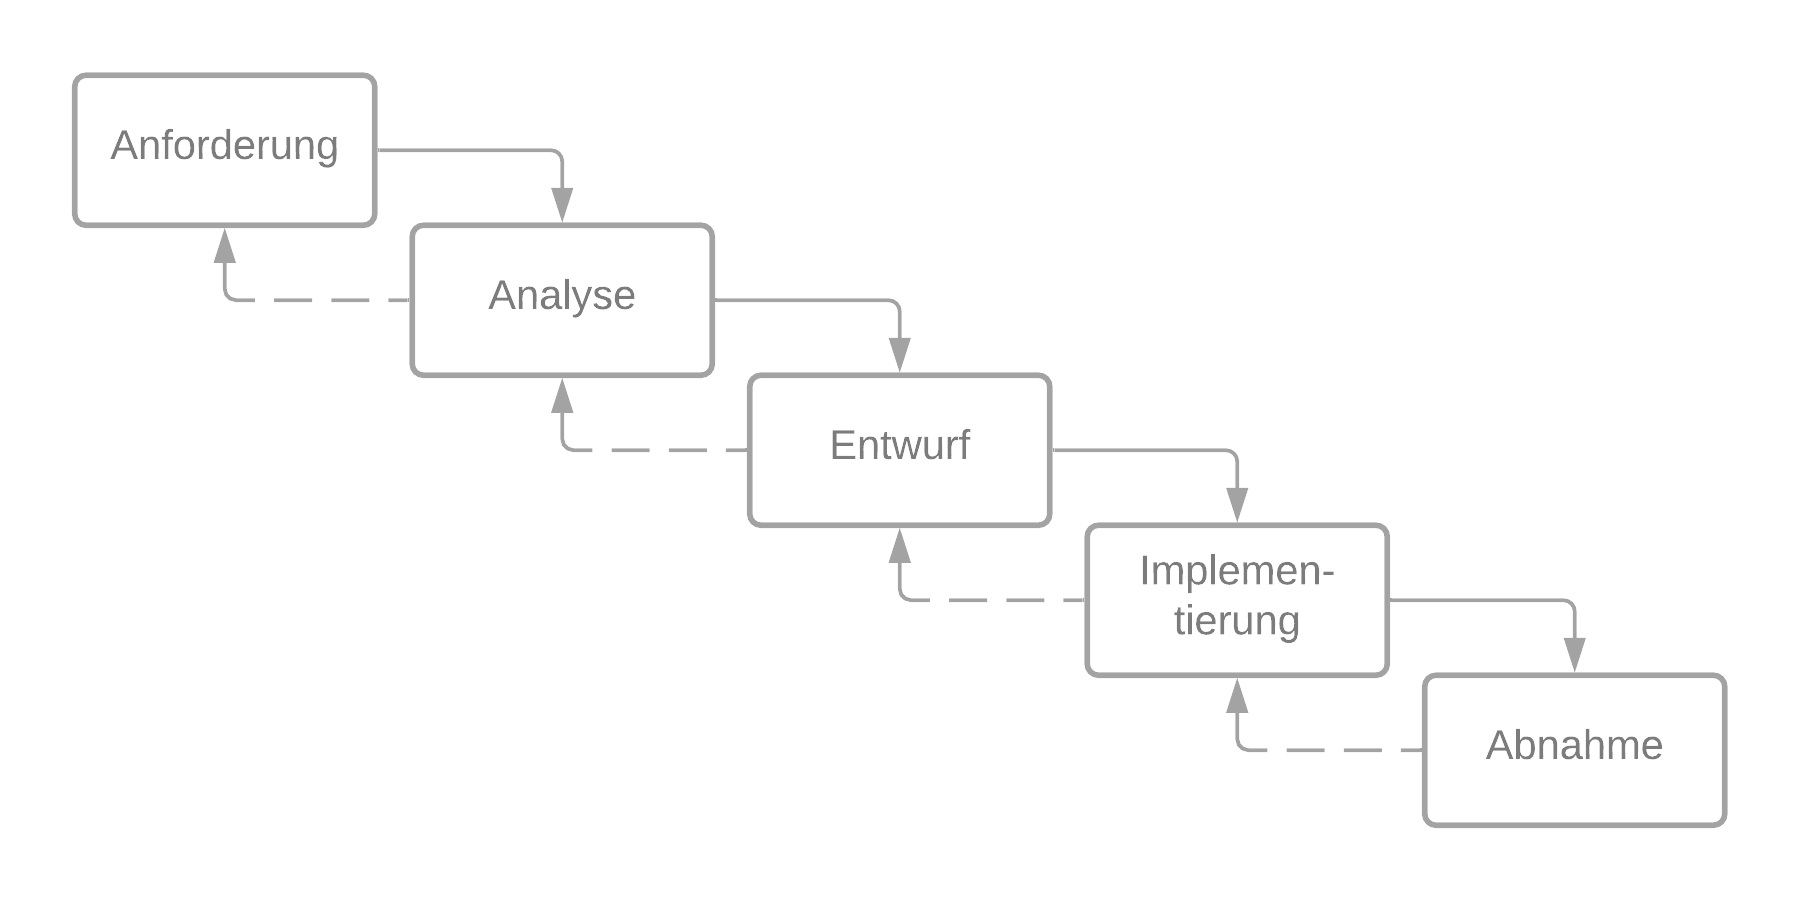
\includegraphics[width=0.55\textwidth]{Wasserfallmodell.png}
      \caption{Erweitertes Wasserfallmodell}
      \label{abb:vg}
    \end{figure}
    \\
    Im weiteren soll der Entwicklungsprozess durch das Test-Driven-Development-Prinzip erweitert werden.
    \newpage
    \subsubsection{Test Driven Developtment}
      Das Test-Driven-Development-Prinzip wird durch die drei folgenden Schritte beschrieben.
        \begin{itemize}
          \item \textbf{Tests erstellen:} Zu Beginn der Implementierung werden Tests erstellt, welche die Funktionalität der neuen Funktion verifizieren sollen.
          \item \textbf{Implementierung:} Die Geschäftslogik hinter den Funktionen implementieren, bis die Tests erfolgreich durchlaufen werden.
          \item \textbf{Refactoring:} Nachdem die Geschäftslogik implementiert wurde, kann der Entwickler seinen Code noch optimieren. 
        \end{itemize}
  \subsection{Projektphasen}\label{sec:plan:phase}
    Durch den gewählten Entwicklungsprozess aus Abschnitt \ref{sec:dev:prc} wurden die zu verfügung stehenden 70 Entwicklerstunden auf die verschiedenen Projektphasen aufgeteilt.
    Die Zeiteinteilung sowie die einzelne Projektphasen wurden für einen groben Überblick in der Tabelle \ref{tab:timing:overview} zusammengefasst.
    Eine genaue Zeitplanung inklusive der Aufgaben in jeder einzelnen Phase können aus dem Anhang \ref{sec:detailTime} entnommen werden. 
    \begin{table}[ht]
      
      \centering
    \begin{tabular}{| l | r |}
      \hline
      \rowcolor{carolinablue}
      Projektphase & Stunden \\
      \hline
      Analysephase & 7h \\
      \hline
      \rowcolor{lightgray}
      Entwurfsphase & 11h\\
      \hline
      Implementierungsphase & 35h\\
      \hline
      \rowcolor{lightgray}
      Abnahme und Testphase & 3h\\
      \hline
      Dokumentation & 14h \\
      \hline
      \rowcolor{carolinablue}
      Gesamtstunden & 70h\\
      \hline
    \end{tabular}
    \caption{Grobe Zeitplanung}
    \label{tab:timing:overview}
  \end{table}  
  \subsection{Ressourcenplanung}
    Das Projekt wurde auf einem, von dem Ausbildungsbetrieb zur Verfügung gestellten, Windows Surface Book geplant, bearbeitet und getestet. 
    Dabei wurde als Entwicklungsumgebung für den TransaltionService sowie für den Java Dienst die Software IntelliJ Ultimate von der Firma JetBrains verwendet. 
    Die Grundlage der Daten für den TranslationSerivce sind in einer MySql Datenbank gespeichert. 
    Zur Überprüfung der korrekten Anwendung des ORM Frameworks Doctrine hinsichtlich DDL, DCL und DML, 
    wurden die Ergebnisse über die Software MySQL Workbench mittels SQL Abfragen validiert. 
    Neben den automatisierten Tests der Schnittstellen mit PHPUnit, 
    wurden regelmäßig mit der Software Postman Anfragen an die REST Schnittstellen geschickt.
    Für die, in Latex erstellte, Dokumentation notwendigen Diagramme wurden über den Onlinedienst Lucidchart angefertigt.
    Eine genaue Übersicht aller verwendeten Ressourcen ist im Anhang \ref{sec:resources} Genutzte Ressourcen zu finden.
  \section{Analysephase}
  \subsection{Ist-Analyse}\label{sec:analyse:current}
    In der nachfolgenden Analyse wird das Kassensystem OktoPOS Cash und der Übersetzungsdienst TranslationService in ihrer ursprünglichen Verfassung beschrieben.
  \subsubsection{OkotoPOS Cash}\label{sec:analyse:current:cash}
    Wie in den Abschnitten \ref{sec:projectdesc} und \ref{sec:projectEnv} beschrieben unterstützt das Kassensystem OktoPOS Cash ein multilinguales Front-End.
    Um das zu gewährleisten, werden im Quellcode der Kasse sog. Übersetzungstokens verwendet. Für jede unterstützte Sprache ist eine Übersetzungsdatei im Property-Format
    in der Ressourcen der Kassesoftware hinterlegt. Im Normalfall sollte jede Datei das gleiche Set an Tokens mit der jeweiligen Übersetzung als Schlüssel-Werte-Paar beinhalten. 
    Bei der Einführung eines neuen Tokens hat der Entwickler die Aufgabe den neuen Token in eine dieser Dateien zu überführen und eine exemplarische Übersetzung anzulegen.
    Da es im Unternehmen gängig ist, die Tokens nur in eine bzw. maximal zwei Dateien zu überführen, wird die Aufgabe der Wartung und Pflege an 
    die Übersetzungsabteilung delegiert. Neben der trivialen und zeitaufwändigen Arbeit die einzelnen Dateien auf den gleichen Stand zu halten,
    kann es auf Grund von diversen Faktoren passieren, dass der Stand der Dateien divergiert.\\
    Bisher gibt es keine benutzerfreundliche Oberfläche, um Übersetzungen für die einzelnen Tokens anzufertigen bzw. auch keine direkte Referenz auf die Textstelle 
    an denen der Token eingesetzt wird. Der Übersetzer hat die Aufgabe, sich aus geeigneten Quellen (Ticketsystem, andere Übersetzungsdatei, Entwickler fragen), eine geeignete Übersetzung
    zu beschaffen. Es gibt allerdings auch Fälle, bei denen keine Übersetzung für einen Token erstellt wurde. Dann hat der Übersetzer die Aufgabe, 
    über das Lesen von Quellcode die konkrete Textstelle im Front-End zu finden.\\
    Im aktuellen Workflow werden die Übersetzungsdatein im Betazustand einer neuen Minor-Version an die Abteilung für Übersetzung übergeben. Nach Fertigstellung
    der Übersetzung werden die überarbeiteten Dateien an den Projekteigentümer der Kassesoftware übergeben, welche er dann mit den alten Übersetzungsdateien zusammenführt.
    Dadurch kann nur noch indirekt über einen Release-Branch auf die verwendeten Übersetzungen geschlossen werden und nicht über einen eigenen Versionsstand der Übersetzungsdateien. 
    Außerdem hat der Workflow zur Folge, dass Änderungen an den Übersetzungsdateien immer ein Versionsupdate der Kasse mit sich bringen.\\
  \subsubsection{TranslationService}\label{sec:analyse:current:ts}
    Für die Übersetzungen in einem anderen System des Unternehmens wurde der webbasierte Transaltionservice entwickelt. 
    Dieser hat die Aufgabe über Http-Schnittstellen, Tokens zu importieren bzw. zu exportieren.
    In einer benutzerfreundlicher Übersicht hat der Übersetzer die Möglichkeit sich nicht übersetzte Tokens für seine Sprache anzeigen zu lassen.
    Neben der Übersicht hat jeder Token, falls vorhanden, eine exemplarische Übersetzung für jede Sprache, in der Token bereits übersetzt wurde.
    Der TranslationService bietet verschiedene Möglichkeiten, die Informationen für Tokens anzeigen zu lassen. 
    Das Komponentendiagramm im Anhang \ref{sec:is:comp} stellt die Beziehungen zwischen den einzelnen Systemkomponenten dar.\\
    Die Daten des Übersetzungsdiensts sind in einer MySql Datenbank gespeichert. Das ERD im Anhang \ref{sec:erd:is} zeigt das Datenbankschema in der ursprünglichen Form. 
    Mit dem ERD wird die Planung der Anpassungen an der Datenbankstruktur erleichtert.\\
    Nach aktuellem Stand ist es nicht möglich, die einzelnen Tokens und deren Übersetzung über eine Version abzubilden. 
    Das hat zur Folge, dass die Änderungen an den Übersetzungen final sind.
  
  \subsection{Soll-Analyse}
    Durch die Anbindung des Kassensystems an den Transaltionservice soll die Pflege und Wartung der Übersetzungsdateien im Kassensystem nahezu automatisiert werden. 
    Die Übersetzungen für die einzelnen Tokens sollen über eine neue Schnittstelle am TranslationService in Abhängigkeit zu ihrer Version bereitgestellt werden. 
    Es ist ein Dienst zu erstellen, welcher die vom TranslationService bereitgestellten Daten an der Schnittstelle anfragt und die Übersetzungsdateien im Livebetrieb aktualisieren kann. 
    Änderungen an Übersetzungen, auf Ebene des TranslationService, werden dann durch den Neustart der Kasse übernommen. Durch die neue Anbindung soll der Übersetzungsprozess vollständig von dem Deployment der Kasse entkoppelt werden.
    Damit die Übersetzungen in Abhängigkeit zu ihrer Version erstellt bzw. bereit gestellt werden können, ist es notwendig den TranslationService hinsichtlich einer Versionierung von Tokens und Translations anzupassen. 
    Die dafür notwendigen Änderungen sind auf Datenbank-, Schnittstellen- und Front-End-Ebene auszuführen.
  \subsection{Wirtschaftlichkeitsanalyse}
  \subsubsection{''Make-Or-Buy''-Entscheidung}
    Da es sich bei dem Projekt um ein internes Feature mit Berührungspunkten an unternehmensinternen Projekten handelt, lässt sich auf dem Markt keine
    alternative Lösung finden. Aus diesem Grund hat man sich dazu entschlossen, das Feature in Eigenentwicklung 
  \subsubsection{Kostenaufstellung}\label{sec:costs}
    In der Tabelle \ref{tab:costs} werden die Kosten, die für dieses Projekt aufgebracht wurden, aufgelistet.
    Entwicklerstunden eines Auszubildenden werden mit 40€ pro Stunde berechnet, während ausgelernte Anwendungsentwickler mit einem Stundensatz von 120€
    veranschlagt werden. In den Kosten ist der Gemeinkostenzuschlag bereits eingerechnet.\\
    \begin{table}[ht]
      \centering
      \begin{tabular}{l l c r r}
        \hline
        \rowcolor{carolinablue}
        Vorgang & Mitarbeiter & Zeit(h)/Mitarbeiter & Personal/h & Gesamt\\
        Entwicklungskosten & 1x Auszubildender & 70h & 40€ & 2800€\\
        \rowcolor{lightgray}
        Planungsmeeting & 2x Anwendungsentwickler & 4h & 120€ & 960€\\
        Codereview & 1x Anwendungsentwickler & 1h & 120€ & 120€\\
        \rowcolor{lightgray}
        Abnahme & 2x Anwendungsentwickler & 0.5h & 120€ & 120€ \\
        \hline
        \rowcolor{carolinablue}
        \textbf{Projektkosten gesamt} &&&& 4000€\\
        \hline
      \end{tabular}
      \caption{Kostenaufstellung}
      \label{tab:costs}
    \end{table}
  \subsubsection{Amortisationsdauer}
    Das Projekt enthält neben den monetäre  Vorteilen auch nicht-monetäre  Vorteile. Daher ist eine genaue Amortisationsdauer nicht festzulegen.
    Dennoch kann anhand der monetäre Vorteile davon ausgegangen werden, dass sich die Anpassungen zu einem späteren Zeitpunkt positiv auf den Gewinn des 
    Unternehmens auswirken.
    \subsubsection{Monetäre Vorteile}\label{sec:MV}
    Nach Abschluss des Projektes werden die Übersetzungsdateien durch den Übersetzungsdienst generiert, 
    die zeitaufwändige Wartung und Pflege entfällt. 
    Durch die benutzerfreundliche Oberfläche des Übersetzungsdiensts müssen externe Übersetzer 
    nicht mehr in die Struktur und Funktionsweise der Übersetzungsdateien eingebarbeitet werden. Die dadurch entstandene Zeitersparnis 
    kann als zusätzlicher Gewinn für das Unternehmen gerechnet werden.
  \subsubsection{Nicht-monetäre Vorteile}\label{sec:notMV}
    Als Softwarehersteller ist der Kundensupport und die Kundenzufriedenheit ein wichtiger Bestandteil der wettbewerbsfähigkeit.
    %% NEU BEGIN
    Auch wenn mit dem Liveupdate der Übersetzungen im Kassensystem und die Versionierung der Tokens 
    und Übersetzungen im TranslationService kann keine konkreten Gewinne berechnen lassen,
    ergeben sich dennoch Voreile, die sich indirekt positiv auf den Unternehmensgewinn auswirken. 
    %% END
  \subsection{Anwendungsfälle}\label{sec:analyse:stakeholder}
    Die Tabelle \ref{tab:stakeholder} zeigt, welche Stakeholder von der Anbindung des Kassensystems an den TranslationService betroffen sind. 
    Das Use-Case-Diagramm im Anhang \ref{sec:uml:uscas} verdeutlicht die direkten Berührungpunkte der Stakeholder mit den Systemen. 
    Da es sich bei dem Projekt um ein internes Feature handelt, wird der Stakeholder "Kunde" nicht mit aufgeführt.
    \begin{table}[ht]
      \begin{tabular}{l l}
        \hline
        \rowcolor{carolinablue}
        Stakeholder & Aufgabenbereich\\
        Übersetzer & Fertig Übersetzungen am Transaltionservice an.\\
        \rowcolor{lightgray}
        Entwickler & Legt im Rahmen eines neuen Features einen neuen Übersetzungstoken an.\\
      \end{tabular}
      \caption{Stakeholder}
      \label{tab:stakeholder}
    \end{table}
  \subsection{Lastenheft}
    Zum Ende der Analyse wurde in Kooperation mit den Verantwortlichen aus den zuständigen Abteilungen ein Lastenheft angefertigt. Dieses beschreibt
    die funktionalen und nicht-funktionalen Anforderungen an das Projekt. Der Abschnitt über die funktionalen Anforderungen ist im Anhang \ref{sec:lastenheft}.
  \section{Entwurfsphase}
    \subsection{Zielplattform}\label{sec:dr:target}
      Das Ziel des Projektes ist, wie im Abschnitt \secref{sec:projectdesc} beschrieben, die Kommunikation zwischen zwei bestehenden System zu ermöglichen.
      Nach Angaben des Auftraggebers aus dem Lastenheft soll die Integrität des Kassencodes bestehen bleiben. Um das zu gewährleisten werden die notwendigen Programmschritte in einen 
      eigenenständigen Dienst ausgelagert.\\
      Als Anforderung an den Dienst soll die Möglichkeit bestehen, diesen zu einem späteren Zeitpunkt in den Kassencode zu integrieren. Daraus entsteht die
      Vorgabe, das Modul auf dem gleichen Java Languagelevel des Kassencodes zu programmieren. %LASTENHEFT\\
      Zum aktuellen Zeitpunkt wird die Kasse über das Build-Management-Tool Ant gebaut. Basierend auf der Anforderung des Auftraggebers %LASTENHEFT%,
      wird in naher Zukunft auf das Build-Management-Tool Gradle umgestellt. Für eine erleichterte Integration des neuen Moduls, soll das neue Projekt bereits den Gradle 
      Buildprozess unterstützen.\\
      Der TranslationService ist in der Programmiersprache PHP auf dem Languagelevel 7.2 programmiert. Es wurde bei der Entwicklung des TranslationService darauf geachtete,
      dass der Service in allen gängigen Webbrowsern\footnote{Mozilla Firefox, Google Chrome, Micrsoft Edge, Safari, Opera} funktionsfähig ist. Für die Darstellung der Daten wird HTML 5.2 verwendet. 
      Für eine klare, ansprechende und benutzerfreundliche Darstellung der Daten wurde das, in HTML 5.2 beschriebene, Front-End mit dem Stylesheet von Twitter Bootstrap verbessert.\\%WORT HIER
      Da es sich bei den Systemen um produktive Systeme handelt, sind die zu benutzenden Programmierparadigmen und Programmiersprachen vorgegeben.
      Das Aufstellen einer Nutzwertanalyse ist daher obsolet.
    \subsection{Architektur}\label{sec:architecture}
      Der TransaltionSerivce basiert auf dem Model-View-Controller (MVC)-Architekturmuster. Demnach werden die zugrunde liegenden Daten in einer Datenbank gespeichert, während die View für
      die Darstellung der Daten verantwortlich ist. Über Controller wird eine bidirektionale Kommunikationschicht geschaffen, um Daten zu manipulieren bzw. Daten anzuzeigen.
      Durch die Entkopplung, welche durch das MVC-Pattern erreicht wird, wird die Erweiter- und Wartbarkeit signifikant erleichtert.\\
      Die Darstellung der Daten im TranslationService wird durch die Template-Engine Twig realisiert. Dabei werden die Daten über Action Klassen der Engine zur Verfügung gestellt.
      Die Twig-Engine verwendet die Daten, um variable Felder mit Daten zu beschreiben. Die Action-Klassen repräsentieren im MVC-Pattern die Controller. Action-Klassen werden üblicherweise über %SATZ TWIG
      vordefinierte Routen aufgerufen und verarbeiten die mitgesendeten Daten auf Grundlage konzipierten Aufgabe. 
      In dieser webbasierten Anwendung werden die genutzten Daten in einer Datenbank persistiert. Die Modelle der Daten sind als Entitäten in einer Datenbank definiert.
      Das Object-Relation Mapping (ORM)-Framework Doctrine automatisiert dabei die Aufgabe, aus definierten Objekten die korrekte DDL zu generieren und auf der Datenbank auszuführen.\\ 
      Die aktuell verwendeten Schnittstellen des TranslationService sind bereits nach der RESTful-Architektur designed. RESTful steht für eine zustandslose 
      Kommunikation zwischen Client und Server. Durch cachingfähige Daten können Client-Server-Interaktionen optimiert werden. 
      Die neuen Schnittstellen, sollen ebenfalls nach der RESTful-Architektur implementiert werden.  
      Der Translationupdater ist der neue Dienst welcher das Kassensystem um eine Subroutine erweitern soll. Die Subroutine beschafft Daten von einem autarkem System, verarbeitet diese 
      und injiziert die verarbeiten Daten in das bestehende Kassensystem.
    \subsection{Benutzeroberfläche}\label{sec:dr:ui}
    Änderungen an der Benutzeroberfläche des TranslationService werden über die Template-Engine Twig durchgeführt. Dabei wird die Oberfläche durch die Auszeichnungssprache HTML beschrieben. Twig bietet die Möglichkeit
    HTML Formulare durch algorithmische Grundstrukturen zu erweitern. Dabei ist es möglich, Iterationen und bedingte Anweisungen direkt im HTML Formular einzubinden.
    \subsection{Datengrundlage}
      Wie im Abschnitt \ref{sec:architecture} beschrieben, persistiert der TranslationService seine Daten nach dem Datenbankschema \ref{sec:erd:is}, in einer MySql Datenbank.
      Die REST Schnittstellen im TransaltionService verwenden das für REST typische Format JSON, um Daten mit Clients auszutauschen. Die neu zu entwicklenden Schnittstellen 
      sollen sich der bestehenden Struktur anpassen und dasselbe Format für den Datenaustausch mit den Clients verwenden.\\
      Als Datengrundlage für die Übersetzungsdateien nutzt das Kassensystem Dateien im Property-Format. Der Translationupdater hat somit auch die Aufgabe, die empfangenen
      Daten aus dem Json-Format in das, von der Kasssensoftware, lesbare Property-Format zu konvertieren.
  \subsection{RESTful APIs}
      Im Abschnitt \nameref{sec:analyse:current:ts} ist beschrieben, dass die bestehenden Schnittstellen nach der REST-Architektur designed wurden. Für eine stringente Implementierung 
      werden neue Schnittstellen ebenfalls nach dem RESTful-Architekturmuster designed. Die Kommunikation zwischen einem Client und einer REST Schnittstelle basiert auf dem HTTP-Request-Response Prinzip.
      Dabei ist der HTTP-Request die Anfrage des HTTP-Client an den Server. Der Server verarbeitet die Anfrage und schickt den HTTP-Response an den Client zurück. 
      Die Abbildung \ref{abb:api:rtr} soll das Prinzip visualisieren.
      \begin{figure}[ht]
        \centering
          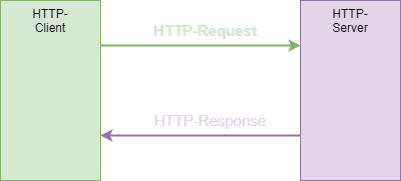
\includegraphics[width=0.5\textwidth]{http-request-response.png}
        \caption{Http-Request-Response-Prinzip}
        \label{abb:api:rtr}
      \end{figure}
      Im Gegensatz zu den ursprünglichen undokumentierten Schnittstellen, hat der Auftraggeber im Lastenheft darum gebten, die neuen Schnittstellen zu dokumentieren.\\
      Als Dokumentationswerkzeug für RESTful APIs wird in diesem Projekt Swagger verwendet. Ein Ausschnitt der, im Planungsmeeting entstandenen, Schnittstellen ist im \attsecref{sec:swa:ts} zu finden.
      Die neuen Schnittstellen wurden in einem Planungsmeeting mit dem zuständigen Projekteigentümer des TranslationServices geplant.
  \subsection{GitWebhook}
      Für die Versionsverwaltung nutzt das Unternehmen den Webanwendung GitLab. GitLab unterstützt die Möglichkeit einen sog. WebHooks einzurichten.\\
      Ein WebHook führt anhand eines bestimmten Ereignis, dir vorgegebenen Anweisungen aus. Für die Anbindung der Kassensoftware an den TranslationSerivce, sollte ein
      WebHook eingerichtet werden, welcher auf ein Merge-Ereignis reagiert. Dabei sollte Änderungen innerhalb der Übersetzungsdateien erkannt und an den TransaltionService weitergeleitet werden.
  \subsection{Testcases}\label{sec:dr:tests}
      Das gesamte Projekt wurde nach dem Prinzip Test-driven entwickelt. Das bedeutet, dass vorangehend zur Implementierung Tests erstellt werden. Die Tests werden auf Grund der fehlenden 
      Funktionalität zu Beginn fehlschlagen. 
      Test-Driven bietet den Vorteil, dass der Entwickler während der Implementierung von Funktionalitäten ein direktes Feedback bekommt, ob das gewünschte Ergebnis erreicht wurde bzw.
      diverse Fehlerfälle aus dem Test abgedeckt wurden.\\
      Damit Tests, die Datenbankzugriffe beinhalten, nicht beeinflusst werden können, werden die Tests auf einer leeren Testdatenbank ausgeführt. Um eine leere Testdatenbank zu garantieren, 
      wird vor und nach jedem Test die gesamte Datenbank bereinigt. 
      Für den Test werden ausschließlich im Test definierte Daten verwendet.
      Die Tests für den TranslationService werden mit dem PHP Framework PHPUnit erstellt und regelmäßig ausgeführt. 
      Der Translationupdater nutzt das Testframework JUnit und führt seine Tests über das Gradle Buildscript während des Buildprozesses aus.
  \subsection{Pflichtenheft}
      Zum Ende der Entwurfsphase wurden die Entwürfe in einem Pflichtenheft zusammengefasst. Das Pflichtenheft beschreibt auf Basis des Lastenheftes
      die geplante Umsetzung der Anforderungen.\\
      Das Pflichtenheft wurde von den betroffenen Abteilungen genehmigt und dient als Leitfaden für die Realisierung des Projektes. 
      Im Anhang \ref{sec:pflichtenheft} ist ein Auszug des erstellten Pflichtenheft zu finden.
  \section{Implementierungsphase}
  \subsection{Iterationsplanung}
      Für eine strukturierte Implementierung wurde ein Iterationsplan erstellt. Dieser gibt dem Entwickler eine Überblick über die erforderlichen Schritte
      zur Fertiggestellung des neuen Features. Da es sich um zwei unterschiedliche Systeme handelt, wurden zwei Iterationspläne erstellt. Der Iterationsplan im Anhang \ref{sec:iterationplan:tr} beschreibt
      den Ablauf der Implementierung für den TranslationService, während der Iterationplan \ref{sec:iterationplan:tu} den Ablauf für den Translationupdater beschreibt.
  \subsection{TranslationService}\label{sec:impl:ts}
  \subsubsection{Erweiterung der bestehenden Datenstruktur}\label{sec:impl:db}
    Als Grundlage für die weiterführende Programmierung wurde zu Beginn der Implementierung mit der Erweiterung der Datenstruktur begonnen. Die daraus resultierenden Änderungen an dem Datenbankschema können aus dem 
    Anhang \ref{sec:erd:final} entnommen werden.
    Um die geforderte Versionierung im TranslationService abbilden zu können, musste die neue Entität \lstinline{Version} in das bestehende Datenbankschema eingebunden werden.
    Das ORM Mapping Tool Doctrine kann über Annotations PHP-Klassen in ein Datenbankschema überführen.\\
    Dabei werden Klassen, die in der Datenbank eine Entität repräsentieren sollen, mit der Annotation \lstinline{@ORM\Table} markiert.
    Listing \ref{lst:an:tb} zeigt, wie die Klasse \lstinline{Version.php} als Entität für Doctrine markiert wird.
    \begin{lstlisting}[caption={Annotation für eine Entität},captionpos=b, label= lst:an:tb]
      @ORM\Table (name="version")
    \end{lstlisting}
    Attribute werden für Doctrine ebenfalls über Annotations markiert. Dabei wird die Annotation über das Attribut der Klasse geschrieben.
    \begin{lstlisting}[caption={Annotation für ein Attribut},captionpos=b, label= lst:an:at]
      @ORM\Column (type="string", nullable=false)
    \end{lstlisting} 
    Dabei können neben dem Datentyp auch weitere Parameter wie zum Beispiel \lstinline{nullable=false} gesetzt werden. \lstinline{Nullable} sagt aus, das der Wert in der Spalte 
    nicht null sein darf.\\
    Aus dem finalen ERD (Anhang \ref{sec:erd:final}) sind neben der neuen Basisentität noch die Relationstabellen Token\_Version und Translation\_Version zu erkennen. Relationstabellen werden von Doctrine generiert, wenn
    zwei Tabellen in einer Many-To-Many Beziehung stehen. In der objektorientierten Programmierung werden Many-To-Many Beziehungen über Listen abgebildet. Dabei haben die beiden
    Objekte eine Liste von Instanzen des jeweiligen anderen Objektes als Attribut.\\
    Damit das verwendente ORM Tool die Relationstabellen für die betroffenen Entitäten erstellen kann, werden weitere Annotations benötigt. Listing \ref{sec:lst:mtmA} zeigt an dem Beispiel Token\_Version die Umsetzung einer M:N Beziehung über Doctrine Annotations.
  \subsubsection{Erweitern der Schnittstellen} \label{sec:impl:api}
    Anhand der Schnittstellendefinition \ref{sec:swa:ts} wurden die neuen Schnittstellen im TranslationService implementiert. Der TranslationService wurde auf Basis des Slim Frameworks aufgebaut.
    Über das PHP-File \lstinline{Bootstrap.php} werden mithilfe der Klasse \lstinline{TranslationServiceAppBuilder.php} die Routen für die Schnittstellen in der TranslationService App definiert.
    Neue Routen werden anhand eine simplen Schemas als Route für die App definiert. Die Definition der Routen innerhalb des Slim Frameworks ist wie folgt aufgebaut:
    \begin{lstlisting}[caption={Beispielroute},label=lst:rt:ex, captionpos=b, label=lst:rt:ex]
      $app->post('/api/v1/{foo}/list',Foo::class)
    \end{lstlisting}
    \begin{table}[ht]
      \centering
      \begin{tabular}{l  l }
        \hline
        \rowcolor{carolinablue}
        Befehl & Erläuterung \\
        \hline
        \$app & Konfigurationsklasse für die Transaltionservice Applikation.\\
        \rowcolor{lightgray}
        post & Definition des HTTP Request für die Route.
                          (GET, POST, PUT usw.)\\
        \'/api/\{foo\}/list\' & Definition der Route. Variable Parameter werden in \{\} dargestellt.\\
        \rowcolor{lightgray}
        Foo::class & Die genutzte Action Klasse die aufgerufen werden soll.
      \end{tabular}
      \caption{Übersicht Routenregistrierung in Slim}
      \label{bzz}
    \end{table}
    Die Tabelle \ref{bzz} erklärt die Bestandteile der Routenregistrierung aus Listing \ref{lst:rt:ex}.
    Im Listing \ref{sec:lst:routes} wird die Umsetzung einer Routenregistrierung anhand von zwei, im Rahmen des Projektes erstellten, Routen deutlich gemacht.\\
    Für die neuen Routen wurden dementsprechen neue Action-Klassen entwickelt die die jeweiligen Anforderung an die Routen erfüllt. \\
    Über das verwendente PHP Framework \begin{lstlisting}
      "php-di/slim-bridge": "^1.1.2"
    \end{lstlisting}
    können alle im Service verwendeten Abhängigkeiten in einem Container abgelegt und per Dependency Injection in den verschiedenen Klassen genutzt werden. 
    In den meisten Fällen haben die Action-Klassen Abhängigkeiten zu den verschiedenen Repositoires. 
    Die Abhängigkeiten werden in den Konstruktoren der Actionklasse definiert. Durch die Dependency Injection
    werden bei Aufruf die definierten Abhängigkeit geladen. Dependency Injection hat den weiteren Vorteil, dass zur Laufzeit auf der gleichen
    Instanz eines Objektes gearbeitet wird.\\
    Beim Aufruf einer Action-Klasse wird die Funktion \lstinline{__invoke} mit den Parameter \lstinline{Slim/Request} und \lstinline{Slim/Response} aufgerufen. 
    Innerhalb der \lstinline{__invoke} wird die eigentliche Logik der Action-Klasse ausgeführt. Über die Referenz auf \lstinline{Slim/Request}-Objekt kann der Entwickler auf die im Request stehenden Daten zugreifen.\\ 
    Der Parameter \lstinline{Response} ist eine Referenz auf das Responseobjekt des Routenaufrufes. Dieser wird so manipuliert, dass die Applikation die korrekten Informationen an den aufrufenden Client zurückgibt. 
    Für den Response stehen mehrere Möglichkeiten zur Verfügung, um die Informationen in ein eindeutig lesbares und serialisierbares Ergebnis zu ''verpacken''. 
    In den meisten Fällen wird für den Datenaustausch über RESTful designte Schnittstellen das JSON-Format genutzt. Neben der Information, ob 
    die angeforderte Operation erfolgreich (success) war, wird eine Message und optional auch noch weitere Daten an den Client zurückgegeben.
    Da es sich um eine Referenz handelt, muss das Responseobjekt nicht neu erzeugt werden. Es werden neue Attribute hinzugefügt oder geändert.\\ %Mal sehen
    Der Ablauf von \lstinline{__invoke} Funktionen der Action-Klasse wird in dem Kapitel Geschäftslogik \ref{sec:impl:bl} genauer erläutert. 
    Während des Projektes wurden alle im Anhang \ref{sec:swa:ts} definierten Routen nach dem in diesem Abschnitt beschriebenen Prinzip implementiert.   
  \subsubsection{Geschäftslogik}\label{sec:impl:bl} %PAUSE
    In dem Abschnitt \ref{sec:impl:api} wurde die Erweiterung der Schnittstellen beschrieben, wie die einzelnen Routen mit dem Slim-Framework angelegt und 
    mit einer Geschäftslogik verknüpft werden. Dieser Abschnitt beschreibt den Umgang mit den mitgesendeten Daten hinsichtlich der generellen Routine, die der Bearbeiter
    genutzt hat, um vorhersehbare Fehler abzufangen und das geforderte Ergebnis zu erreichen.\\ 
    Wie im Abschnitt \ref{sec:impl:api} beschrieben, hat jede Route genau eine eigene Action-Klasse, alternativ auch Controller genannt, die wiederrum genau eine \lstinline{__invoke}-Funktion besitzt. Listing \ref{lst:impl:bl:GET} und Listing \ref{lst:impl:bl:POST} 
    zeigen zwei unterschiedliche Implementierungen der \lstinline{__invoke}-Funktionen. Die Implementierung der \lstinline{__invoke}-Funktionen richtet sich nach den Vorgaben der Schnittstellendokumentation im Anhang \ref{sec:swa:ts}.
    Eine \lstinline{__invoke}-Funktion beginnt damit, die mitgesendeten Daten und Routenparameter in geeignete Variablen zu überführen. Um zu verhindern, dass mit 
    fehlenden, falschen oder kaputten Daten gearbeitet wird, werden vor zuerst die - für die Schnittstelle definierten - Fehlerfälle abgefangen und mit dem, in der Schnittstellendokumentation \ref{sec:swa:ts} definierten, Response
    an den Client zurückgegeben.\\
    Nach Ausschluss aller möglichen Fehlerfälle, können die validen Daten verarbeitet werden. Die Erweiterung des TranslationService beinhaltet drei Arten von Schnittstellen - Hinzufügen, Ändern und Abfragen von Daten.
    Die drei genannten Typen der Datenverarbeitung greifen auf die geeigneten Funktionen der Entityrepositories zu. Um die Rechenleistung des Servers zu entlasten, wird die Anzahl der Datenbankoperationen so 
    gering wie möglich gehalten. Um das zu erreichen bietet der Entitymanager von Doctrine die Möglichkeit alle Änderungen erst in einem Cache zu persistieren. Persistierte Änderungen werden 
    über die Funktion \lstinline{$this->_em->flush} des Entitymanager in die Datenbank geschrieben. Als Anwendungsfall gelten Massenimporte von Tokens. Die Tokens werden aus dem Request ausgelesen, validiert, als konkretes Objekt erstellt und in einem Cache hinterlegt.
    Erst nach der vollständigen Iteration über die gelieferten Tokens werden die Änderungen in der Datenbank gespeichert.\\
    In dem Abschnitt \ref{sec:dr:ui} wird der grundlegende Aufbau der Benutzeroberfläche des TranslationService erläutert. Die Anforderungen des Auftraggebers hinsichtlich der 
    Erweiterungen der Benutzeroberfläche beschränken sich auf einen weiteren Filter, der die Translation und Tokenübersicht hinsichtlich ihrer Version sortiert.
    Dabei hat sich der Projektbearbeiter an den bestehenden Style der Benutzeroberfläche gehalten. Im Anhang \ref{sec:impl:ui} ist ein Vorher-Nachher-Vergleich zu sehen.
    Für den neuen Filter wurde ein neuer Dropdown-Button an das bestehende Filtermenu angefügt. Das Dropdown besteht aus den einzelnen Versionen die bereits im System angelegt wurden.
    Die Daten werden dem Front-End über die Twig-Engine bereitgestellt. Der Klick auf ein Dropdown-Item löst die % Bearbeiten wenn wieder fit
  \subsection{Translationupdater}
    Die zweite Iterationsphase des Projektes behandelt die Implementierung des Translationupdaters. Der Translationupdater ist ein Dienst zum Aktualisieren der Übersetzungsdateien der Kassensoftware. 
    Die Routine für den Translationupdater besteht aus drei Teilen - Beschaffung, Verarbeitung, Injektion. Die Routine des Translationupdaters wird nach Vorgaben des erstellten Aktivitätsdiagramm (Anhang \ref{sec:activ}) implementiert. 
    Da es sich um einen Dienst für das Kassensystem handelt, sind bestimmte Parameter über eine Konfigurationsdatei steuerbar. Die Tabelle \ref{tab:impl:tu:config} beschreibt die konfigurierbaren Parameter des neuen Dienstes.
    \begin{table}[ht]
      \centering
      \begin{tabular}{l l}
        \hline
        \rowcolor{carolinablue}
        Parameter & Erläuterung \\
        \hline
        baseUrl & Bestimmt die URL über die der TranslationService erreichbar ist\\
        \rowcolor{lightgray}
        languages & Eine Liste von Sprachen die aktualisiert werden sollen\\
        version & Gibt die Version der Übersetzungen an
      \end{tabular}
      \caption{Konfigurationsparameter}
      \label{tab:impl:tu:config}
    \end{table} 
    Die Konfiguration des Translationupdater wird über die Klasse \lstinline{SystemConfig.java} realisiert. Diese lädt die einzelnen Properties aus der 
    \lstinline{configuration.ini} (siehe Listing \ref{lst:impl:ul:config}) und überführt die Werte der Parameter in Attribute der Klasse. Über eine Instanz
    der \lstinline{SystemConfig.java} können via \lstinline{Getter}-Methoden auf die einzelnen Werte zugegriffen werden. Da es sich bei der Konfiguration um eine 
    eindeutige, zur Laufzeit unveränderbare Klasse handelt, wurde die \lstinline{SystemConfig.java} als Singleton-Pattern implementiert.\par Die Singletonimplementation stellt sicher, dass 
    von einer Klasse genau ein Objekt erzeugt wird. Da eine Konfiguration normalerweise an verschiedene Stellen im Code verwendet wird, kann auch der Vorteil der globale Erreichbarkeit 
    eines Singleton genutzt werden. Listing \ref{sec:lst:singleton} zeigt anhand der \lstinline{SystemConfig.java} wie eine Singletonimplementation umgesetzt wird.\\
    Als weitere Utility wurde das \lstinline{Printer}-Interface geschaffen. Das \lstinline{Printer}-Interface abstrahiert die in der Tabelle \ref{tab:impl:tu:output} gelisteten Methoden um unterschiedliche Implementierung durch verschiedene Printer zuzulassen.
    \begin{table}[ht]
      \centering
      \begin{tabular}{l l}
        \hline
        \rowcolor{carolinablue}
        Signatur & Beschreibung \\
        \hline
        \multirow{2}{*}{printProgressMessage(int progress, int max, String toWrite)} & Gibt den aktuellen Progress \\ & inklusive einer Nachricht aus\\
        \rowcolor{lightgray}
        print(String message) & Gibt Nachricht aus.\\
        printError(String error) & Gibt einen Error aus.\\
        \rowcolor{lightgray}
        printWarning(String) & Gibt eine Warnung aus.
      \end{tabular}
      \caption{Printer Interface}
      \label{tab:impl:tu:output}
    \end{table}
    Eine konkrete Implementierung des \lstinline{Printer}-Interfaces ist die Klasse \lstinline{ConsolePrinter.java}. Der \lstinline{ConsolePriner} soll die Nachrichten über
    die Kommandozeile an den Nutzer weitergeben. Durch das Interface \lstinline{Printer.java} besteht die Möglichkeiten zu einem anderen Zeitpunkt weitere Ausgabeformen zuzulassen.
    Der erste Schritt der eigentlichen Routine, ist die Beschaffung der geforderten Daten von einem autarken System. Der TranslationService stellt die versionierten Übersetzungen über die Schnittstelle (Listing \ref{lst:rt:export:tr})
    \begin{center}
      \begin{lstlisting}[caption={Export Translations}, captionpos=b, label=lst:rt:export:tr]
        '/api/v1/version/{version}/translations/{language}
      \end{lstlisting}
    \end{center}
    Die Schnittstelle erwartet die Parameter \lstinline{version} und \lstinline{language}. Für den Parameter \lstinline{version} ist der Wert aus der \lstinline{SystemConfig.java} zu verwenden.
    In den Anforderungen aus dem Lastenheft an den Translationupdater beschreibt der Auftraggeber, dass die Aktualisierung von mehreren Übersetzungsdateien innerhalb eines Programmaufrufes möglich sein muss.
    Die Konfiguration stellt dafür den überladbaren Parameter \lstinline{languages} bereit. Die \lstinline{SystemConfig.java} gibt die konfigurierten Sprachen mit einem \lstinline{Getter} als Liste von Sprachen zurück.
    Die in Listing \ref{lst:rt:export:tr} beschriebene HTTP-Schnittstelle stellt nur die Übersetzungen einer Sprache bereit. Daher muss die Schnittstelle für jede einzelne Sprache neu angesprochen werden. Die Routine zur Datenbeschaffung ist als
    Nassi-Shneiderman-Diagramm im Anhang \ref{sec:impl:algo:load} beschrieben.\par
    Der notwendige HTTP-GET-Request wird mithilfe der externe Java Library \lstinline{org.apache.httpcomponents} erstellt und ausgeführt. 
    Der Methodenaufruf \lstinline{CloseableHttpClient::execute} gibt eine Referenz auf das Responseobjekt zurück, mit dem die ''Antwort'' des TranslationService ausgelesen werden kann.
    Die Schnittstellendokumentation \ref{sec:swa:ts} beschreibt den Response bei einer erfolgreichen Anfrage. Mit der externen Library \lstinline{com.google.gson} werden die Array-elmente des
    Json in ein Array von Objekten des Elementtypen \lstinline{TransferObject} überführt. Zur weiteren Verwendung der Daten, wird das Array in eine ArrayList umgewandelt und mit dem jeweiligen Sprachenkürzel als Key in einer HashMap hinterlegt.\par
    Im nächsten Schritt der Routine, werden die bereitgestellten Daten in das Property-Format konvertiert und temporär als Datei im Dateisystem abgelegt. Der Dateiname setzt sich aus dem prefix \lstinline{translation}, dem Ländercode z.B. \lstinline{De} und
    der Dateiendung \lstinline{.properties} zusammen.\par
    Der letzte Schritt injiziert die Übersetzungsdateien in die \lstinline{.jar} er Kassensoftware. Der schematische Aufbau der Kassensoftware unterliegt laut der Betriebsordnung der OktoPOS Solutions GmbH
    der Geheimhaltung. Daher ist es dem Autor dieses Dokumentation nicht gestattet, konkrete Informationen über den Zielpfad der Injektion anzugeben. 
    Das Updaten einer .jar-Datei ist innerhalb einer Java-Anwendung nur über externe Hilfsmittel möglich. Im folgenden wird ein ''Workaround'' für die eigentliche Injektion beschrieben.\\ 
    Der \lstinline{CashDeskInjector.java} sucht innerhalb seines Dateiverzeichnis nach der konkreten .jar der Kassensoftware. Wird diese nicht gefunden, wird eine Warnung an den 
    Benutzer ausgegeben und das Programm beendet. Dabei werden die im zweiten Programmschritt erstellten Übersetzungsdateien aus dem Dateisystem gelöscht. In dem anderen Fall wird ein CMD-Befehl generiert, der die Übersetzungsdatei im Klassenpfad der Kasse durch die neue Übersetzungsdatei ersetzt.
    Listing \ref{lst:algo:jarUF} beschreibt den grundlegenden Aufbau des CMD-Befehls der über den Java Befehl \lstinline{Runtime.getRuntime().exec(String command)} ausgeführt wird.
    \begin{lstlisting}[caption={Update Jar},captionpos=b,label=lst:algo:jarUF]
      jar -uf foobar.jar de/foo/resources/translationDe.properties
    \end{lstlisting}
    Nach erfolgreicher Injektion der Übersetzungsdatei, wird diese aus dem Dateisystem entfernt. Nach vollständigen Injektion aller Übersetzungsdateien, wird eine 
    Nachricht an den Nutzer ausgegeben und das Programm beendet.
  \section{Abnahme- und Einführungsphase}
  \subsection{Abnahme durch den Fachbereich}\label{sec:review}
    Die Änderungen am TranslationService wurden nach Fertigstellung dem zuständigen Projekteigentümer vorgelegt. Die Anforderungen und Lösungsansetze wurden in den Meetings 
    regelmäßig besprochen, daher war der Großteil der Änderungen bereits bekannt und die Abnahme konnte innerhalb kurzer Zeit durchgeführt werden.
    Der neu entwickelte Dienst Translationupdater wurde durch den Projekteigentümer der Kassensoftware abgenommen. Dabei wurden Verbesserungsvorschläge bezüglich des iterativen Ablaufes
    der Routine angemerkt und für den Ausblick \ref{sec:future} notiert. 
    
    \subsection{Deployment}
      Nach den Vorgaben des Auftraggebers soll der neue Dienst über den Buildprozess Gradle gebaut werden. Daher wurde das Projekt im Vorfeld über das \lstinline{Gradle Init Plugin}
      als Gradle Projekt angelegt. Im Nachgang wurde das Gradlescipt um die unternehmensinternen Buildparameter erweitert. Für das Deployment des neuen Dienstes wurde
      ein neuer Task auf dem unternehmensinternen Buildserver angelegt.\\ 
      Da es bei dem TranslationService zu Änderungen an bestehenden Entitäten gekommen ist, müssen bestehende Livedaten des Service über ein SQL Script auf das neue Datenbankschema angepasst werden. 
      Damit ein problemloses Update des Livesystems durchgeführt werden kann, muss mit den Kunden der OktoPOS Solutions GmbH ein geeigneter Termin kommuniziert werden.
      Die verschiedenen Faktoren führen dazu, dass die Anbindung des Kassensystems an den TranslationService erst zum Februar des Jahres 2021 durchgeführt werden kann.
    
    \subsection{Schulung der betroffenen Stakeholder}
      Durch die Anbindung der Kassensoftware an den bestehenden TranslationSerivce ändert sich der Workflow zum Erstellen von Übersetzungen. Die betroffenen Stakeholder aus dem Abschnitt \ref{sec:analyse:stakeholder} werden durch eine Präsentation über die Änderungen in Kenntnis gesetzt. 
      Der zuständige Leiter der Übersetzungsabteilung bekommt zusätzlich eine Einweisung in die Arbeit mit versionierten Übersetzungen.
  \section{Retroperspektive}
  \subsection{IST-SOLL-Vergleich}
    Im Rahmen des Projektes wurden zwei der drei Kernziele erreicht. Während der Planung des Projektes wurden von dem Autor Entscheidungen außerhalb seines Zuständigkeitsbereiches getroffen. 
    Durch die Missachtung der Zuständigkeit, mussten die drei geplanten Schnittstellen verworfen werden und wurden durch die sieben neuen ersetzt. Dabei entstand eine eklatante Diskrepanz zwischen 
    der veranschlagten und genutzten Zeit für die Implementierung der Schnittstellen. Der Autor hat in Absprache mit den Verantwortlichen den GitWebhook
    an eine weitere Abteilung ausgelagert.\\
    Ansonsten wurden die Vorgaben aus dem Lastenheft des Auftraggebers erfolgreich ausgeführt. 
    \subsection{Lessons Learned}
    Durch das Abschlussprojekt hat der Autor viele wertvolle Erfahrungen im Bereich der Projektplanung und Durchführung sammeln können. Speziell die fehlende Kommunikation
    mit einem der beiden Fachbereiche hat zu einem Fehler geführt, der von dem Bearbeiter in der Zukunft nicht noch einmal gemacht wird.\\ 
    Neben den bereits umfangreichen Kenntnissen in der Programmiersprache Java konnte der Autor weitere Fähigkeiten im Bereich der Webentwicklung mit PHP und den dazugehörigen Frameworks erwerben. 
    \subsection{Ausblick}\label{sec:future}
    Während der Bearbeitung des Projektes sind bereits weitere Vorschläge für die Verbesserung der TranslationService Anbindung besprochen worden. 
    Wie in dem Abschnitt \ref{sec:dr:target} Zielplattform angeschnitten, soll der Translationupdater später in den Kassencode als Modul integriert werden. Dabei 
    soll die jetzt über eine neue Konfigurationsdatei einstellbaren Parameter durch das Kassensystem vorgegeben werden.\\
    Im Abschnitt \ref{sec:review} hat der zuständige Reviewer die Anmerkung gemacht, die aktuell drei verwendeten Schleifen für den Updateprozess auf 
    eine Schleife zu kürzen.\\
    Der TranslationService bietet noch die Möglichkeit für die verwendenten Tokens eine Position (Datei + Zeile) anzugeben. Für die Zukunft ist geplant, die genutzten 
    Tokens innerhalb des Kassencodes zu lokalisieren und die Daten im Service zu updaten. Dafür wurde ebenfalls der Vorschlag in Betracht gezogen, die Position des
    Übersetzungstokens zu versionieren.
  \newpage
  \setcounter{section}{0}
  \setcounter{page}{1}
  \pagenumbering{roman}
  \renewcommand{\thesection}{\MakeUppercase{\alph{section}}}
  \section{Anhang}
  \subsection{Detaillierte Zeitplanung}\label{sec:detailTime}
  \begin{table}[ht]
    \centering
  \begin{tabular}{l l  r r}
    \hline
      \rowcolor{carolinablue}
      &\textbf{Analysephase} && \textbf{7h} \\
    \hline
      1. & Durchführung der IST-Analyse & 1h & \\
      \rowcolor{lightgray}
      2. & Durchführung der Soll-Analyse & 2h & \\
      3. & Durchführung der Wirtschaftlichkeitsanalyse & 1h & \\
      \rowcolor{lightgray}
      4. & Erstellung des Lastenheftes & 3h\\
      \rowcolor{carolinablue}
      &\textbf{Entwurfsphase} && \textbf{11h} \\
      \hline
      1.& Zielplattform festlegen & 1h &\\
      \rowcolor{lightgray}
      2.& Architektur festlegen & 1h &\\
      3.& Erweiterung der Datenbank entwerfen & 1h &\\
      \rowcolor{lightgray}
      4.& Neue Schnittstellen planen und beschreiben & 2h &\\
      5.& Geschäftslogik für den TranslationService planen &2h  & \\
      \rowcolor{lightgray}
      6.& Anpassungen am Front-End planen & 1h & \\
      7.& Translationupdater planen (Aktivitätsdiagramm) & 2h &\\
      8.& Erstellen des Pflichtenheftes  & 1h&\\
      \rowcolor{carolinablue}
      &\textbf{Implementierungsphase} && \textbf{35h} \\ 
      \hline
      1.& Erweiterung des bestehen Datenbankmodelles & 1h &\\
      \rowcolor{lightgray}
      2.& Implementieren der PHPUnit Tests für die geplanten Schnittstellen & 5h &\\
      3.& Implementieren der neuen Schnittstellen & 12h &\\
      \rowcolor{lightgray}
      4.& Anpassen der bestehenden Benutzeroberfläche & 2h &\\
      5.& Implementieren der Routine nach dem Aktivitätsdiagramm & 2h &\\
      \rowcolor{lightgray}
      5.& Erstellen der Unittests für die einzelnen Komponenten des Java Dienstes & 4h &\\
      6.& Implementieren der Geschäftslogik für den Downloadmanager & 2h  & \\
      \rowcolor{lightgray}
      7.& Implementieren der Geschäftslogik für den TranslationConvertors & 2h &\\
      8.& Implementieren der Geschäftslogik für den CashDeskInjector  & 3h&\\
      \rowcolor{lightgray}
      9.& Erstellen des GitWebhooks zum Senden der verwendeten Tokens an den Service  & 2 &\\
      \rowcolor{carolinablue}
      &\textbf{Abnahme- und Testphase} && \textbf{7h} \\ 
      \hline
      1.& Testen der Schnittstellen mit Postman & 3h &\\
      \rowcolor{lightgray}
      2.& Abnahme des TranslationService durch den zuständigen Anwendungsentwickler & 1h &\\
      3.& Testen der Funktionalität des Translationupdater & 2h &\\
      \rowcolor{lightgray}
      4.& Abnahme des Translationupdater durch den zuständigen Anwendungsentwickler & 1h &\\
      \rowcolor{carolinablue}
      &\textbf{Dokumentation} && \textbf{14h} \\
      \hline
      1.& Erstellen der Projektdokumentation &12h &\\
      \rowcolor{lightgray}
      2.& Erstellen der Entwicklerdokumentation &2h&\\
      &\textbf{Gesamt} && \textbf{70h} \\
  \end{tabular}
  \caption{Detaillierte Zeiteinteilung}
\end{table}  
\newpage
\subsection{Komponentendiagramm TranslationService}\label{sec:is:comp}
\begin{figure}[htb]
  \centering
  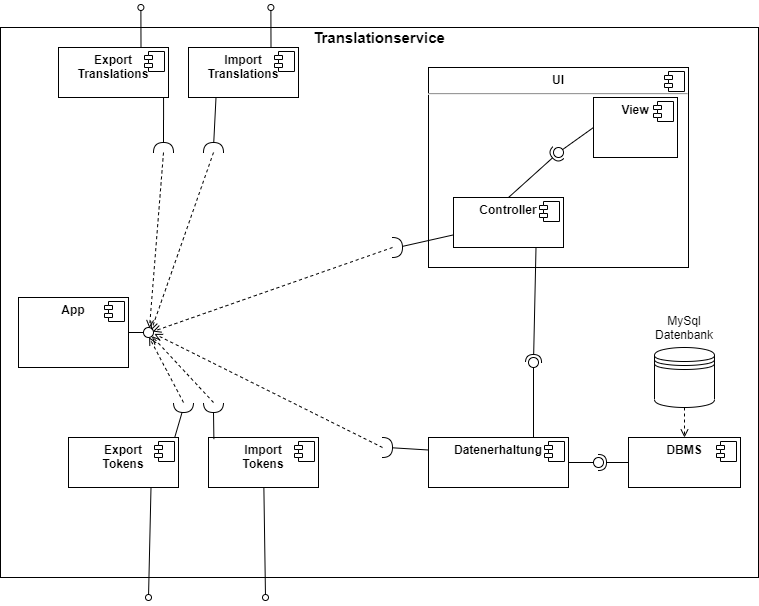
\includegraphics[width=\textwidth]{KomponentenDiagramm.png}
  \caption{Komponentendiagramm TranslationService}
\end{figure}
\newpage
\subsection{Use-Case-Diagramm}\label{sec:uml:uscas}
\begin{figure}[htb]
  \centering
  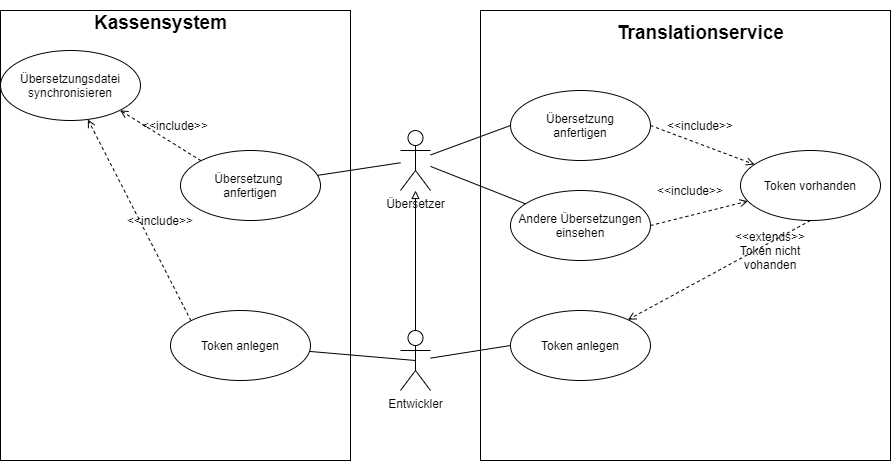
\includegraphics[width=\textwidth]{Use-Case-Diagramm.png}
  \caption{Use Case Diagramm Übersetzungen}
\end{figure}
\newpage
\subsection{Datenbankstruktur Urfassung}\label{sec:erd:is}
  \begin{figure}[htb]
    \centering
    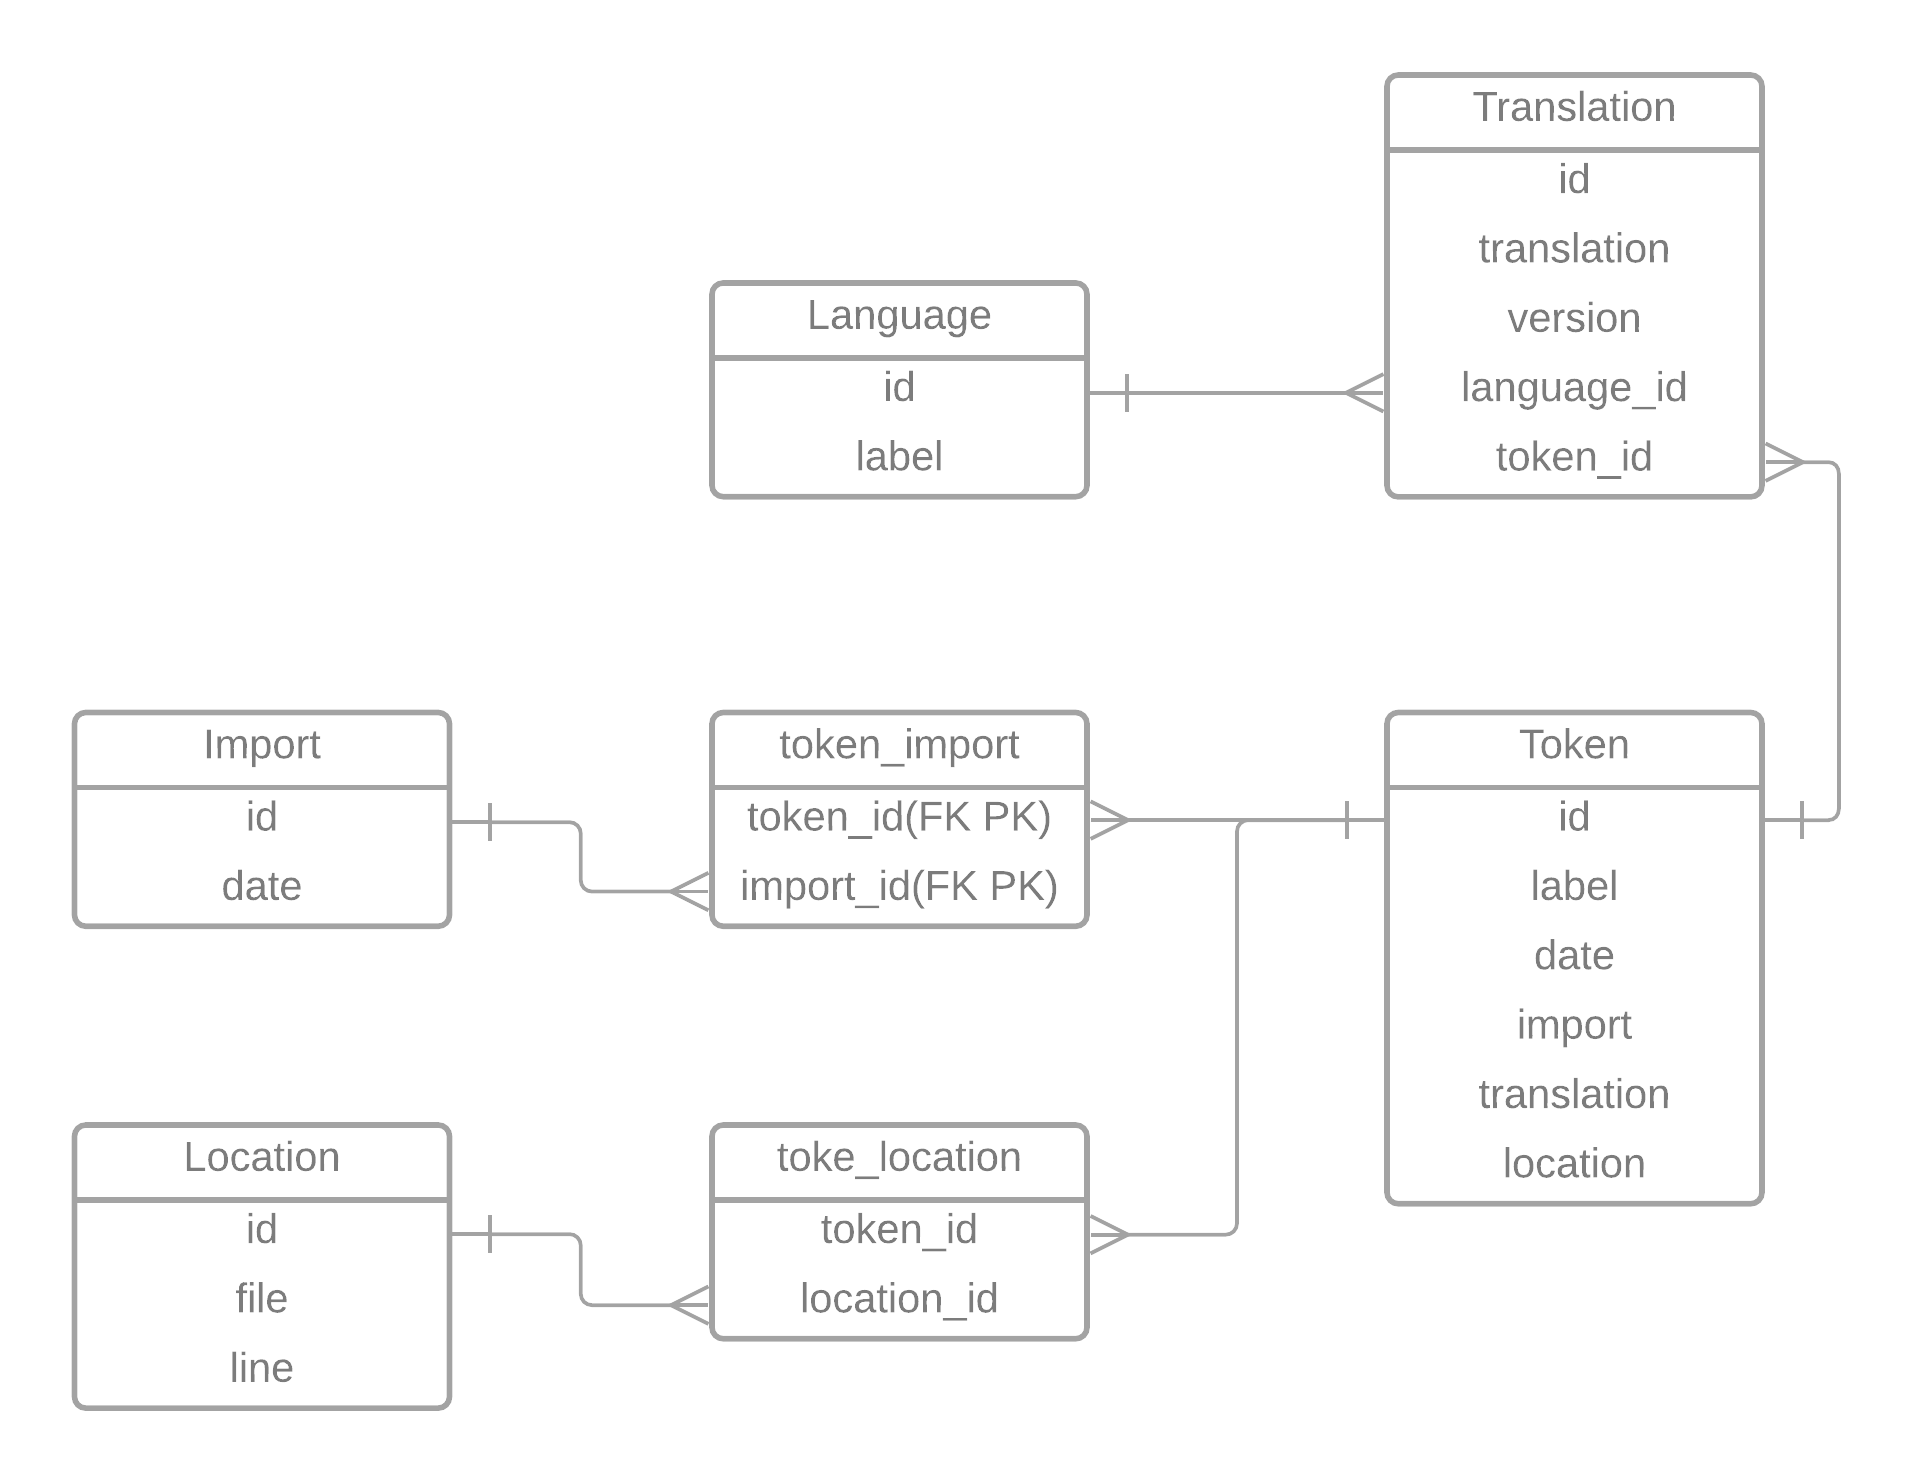
\includegraphics[width=0.7\textwidth]{ERD_TranslationService_IST-Analyse.png}
    \caption{ERD im IST Zustand}
  \end{figure}
\subsection{Finale Datenbankstruktur}\label{sec:erd:final}
  \begin{figure}[ht]
    \label{abb:erd:final}
    \centering
    \includegraphics[width=0.7\textwidth]{ERD_TranslationService_Soll-Analyse.png}
    \caption{ERD im Soll Zustand}
  \end{figure}
  \newpage
\subsection{Ressourcen und Technologien}\label{sec:resources}
  \begin{table}[ht]
    \begin{tabular}{ l  l }
      \hline
      \rowcolor{carolinablue}
      \textbf{Hardware} & \\
      & Microsoft Surface Book - Entwicklungsrechner\\
      & \\
      \hline
      \rowcolor{carolinablue}
      \textbf{Software} & \\
      \hline
      & Microsoft Windows 10 - Betriebssystem\\
      &  \\
      \multirow{2}{*}{ }& JetBrains IntelliJ Ultimate 2020.2  - Entwicklungsumgebung\\ &für den TranslationService und Translationupdater\\
      & \\
      & MySql Workbench 8.0 CE - Datenbankmanagement und SQL Abfragen\\
      & \\
      & Postman 7.36.0 - Erstellen von HTTP Requests\\
      & \\
      & Laragon 4.0.16 - Lokale Webserverumgebung\\
      & \\
      & TexLive V. 2020 - Distribution des Textsatzsystem \LaTeX\\
      & \\
      & Visual Studio code - Editor zum Erstellen der Dokumentation in \LaTeX\\
      & \\
      & Lucidchart - Webanwendung zum Erstellen von UMl-Diagrammen und Grafiken\\
      &\\
      & Draw.io - Webanwendung zum Erstellen von UMl-Diagrammen und Grafiken\\
      \hline
      \rowcolor{carolinablue}
      \textbf{Personal} & \\
        & Entwickler - Umsetzung des Projektes\\
        & \\
        & Projektverantwortlicher TranslationSerivce - Planungsmeeting und Codereview\\
        & \\
        & Projektverantwortlicher Kassensystem - Planungsmeeting und Codereview\\
    \end{tabular}
    \caption{Genutzte Ressourcen}
  \end{table}
    \newpage
  \subsection{Lastenheft}\label{sec:lastenheft}
  Im folgenden Auszug aus dem Lastenheft werden die Anforderungen definiert, die die zu entwickelnde
  Anwendung erfüllen muss.
  \section*{Lastenheft}
  \begin{itemize}
    \item Der TranslationService muss die Möglichkeit bieten Tokens und Translations versioniert abzuspeichern. Dabei gilt: Ein Token kann in mehreren Versionen enthalten sowie eine Version kann aus mehreren Token bestehen. Gleiches gilt für die Translations.
    \item Es muss eine neue Schnittstelle geschaffen werden, die es ermöglicht von außen eine neue Version anzulegen.
    \item Es müssen neue Schnittstelle geschaffen werden, die es ermöglichen Tokens und Translations einer Version hinzuzufügen.
    \item Für einen ''Massenimport'' an Translations und Tokens sollen die jeweils neuen Schnittstellen einen Diff zu einer gewählten Version erstellen. 
    Dabei sollen nicht verwendete Tokens/Translations aus der Version entfernt werden.
    \item Es müssen neue Schnittstelle geschaffen werden, welche den Export von Tokens und Translations in Abhängigkeit zu einer Version ermöglichen.
    \item Die Translation- und Tokenübersicht soll einen neues Dropdown-Menu erhalten, mit dem die Tokens/Translations anhand der Version gefiltert werden können.
    \item Das Übersetzungsdateien innerhalb des Kassensystems sollen im Livebetrieb aktualisiert werden.
    \item Im Rahmen des Projektes ist die Integrität des Kassencodes zu erhalten. Daher soll das Update der Übersetzungsdateien über einen externen Dienst durchgeführt werden.
    \item Der externe Dienst soll so vorbereitet werden, dass er ohne weiteres in den Kassencode integriert werden kann.
    \item Neu angelegte Tokens sollen den TranslationService gesendet werden, sobald ein neues Feature zum Testen freigegeben wurde.
    \item Das Projekt soll über den Buildprozess Gradle gebaut werden.
  \end{itemize}
  \vspace{2cm}
  \begin{center}
    [...]
  \end{center}
  \newpage
  \subsection{Schnittstellendokumentation Auszug}\label{sec:swa:ts}
  \begin{figure}[htb]
    \centering
    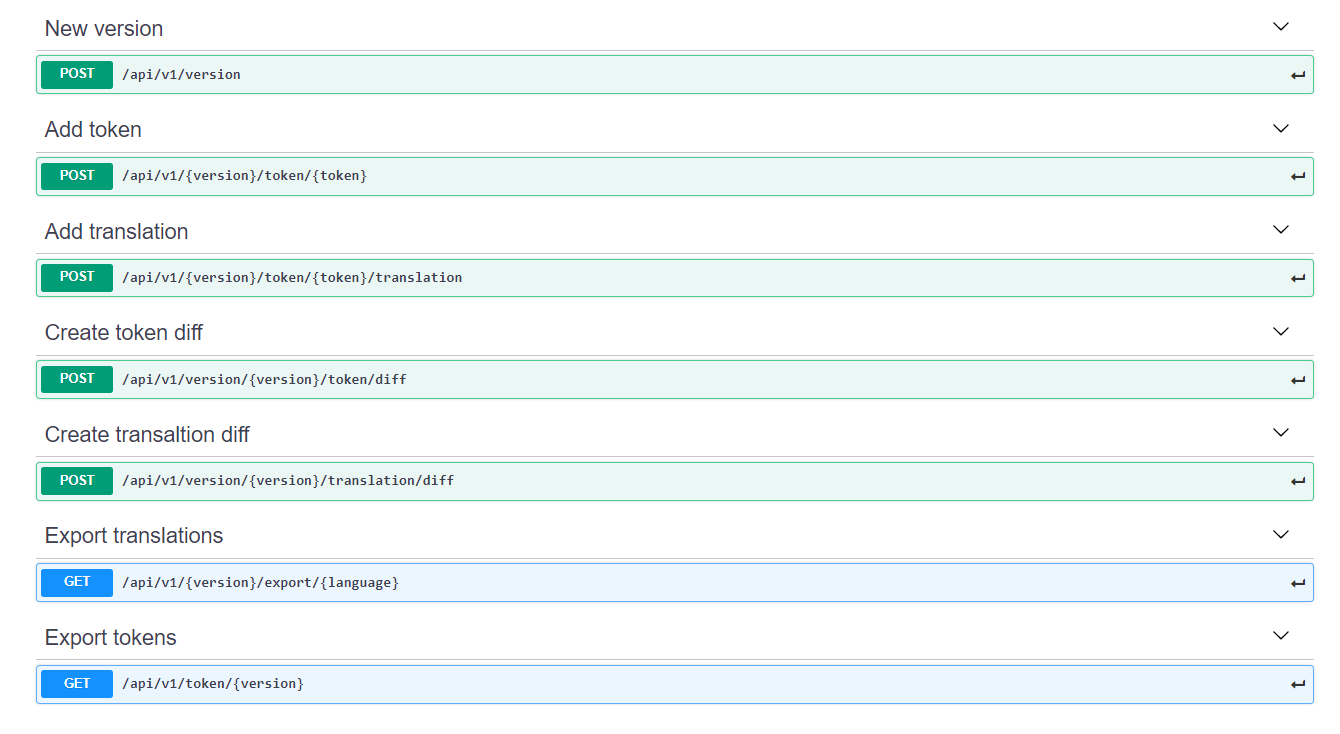
\includegraphics[width=\textwidth]{Swagger_API_Overview.PNG}
    \caption{Übersicht der geplanten Schnittstellen}
  \end{figure}
  \newpage
  \subsection{Pflichtenheft}\label{sec:pflichtenheft}
  In folgendem Auszug aus dem Pflichtenheft wird die geplante Umsetzung der im Lastenheft definierten
  Anforderungen beschrieben:\\ \\
  \subsection*{Umsetzung der Anforderungen}
  \begin{itemize}
    \item Damit Tokens und Transaltions versioniert werden können ist eine weitere Entität in der Datenbank notwendig. 
    Ohne weitere Relationstabellen zwischen den Version und Translation bzw. Version und Token würde das Datenbankschema nicht mehr in er 3ten Normalform sein. 
    \item Diverse neue Schnittstellen werden nach der Schnittstellendokumentation basierend auf der RESTful Architektur designed und implementiert.
    \item Die Anpassungen am Front-End werden auf Basis des bisherigen Styles des TranslationService ausgeführt.
    \item Der neue Dienst zum Updaten der Übersetzungsdateien wird in der gleichen Java Version entwickelt in dem auch die Kasse entwickelt wurde.
    \item Damit ein neues Feature von der Qualitätsmanagement-Abteilung getestet werden kann, wird der Feature-Branch in den Masterbranch gemerged. Um die Vorgabe zu erfüllen die neuen Tokens an den TranslationService zu übergeben,
    wird zum Zeitpunkt des Merges der GitWebhook ausgelöst und sendet die neuen Token an den Service.
  \end{itemize}
  \vspace{2cm}
  \begin{center}
    [...]
  \end{center}
  \newpage
  \subsection{Iterationsplan TranslationService}\label{sec:iterationplan:tr}
  \begin{itemize}
    \item Erweitern des Datenbankschemas
    \item Hinzufügen der neuen Schnittstellen
    \item Implementieren der Geschäftslogik für die Schnittstellen
    \item Anpassen des Front-Ends
  \end{itemize}
  \subsection{Iterationsplan Translationupdater}\label{sec:iterationplan:tu}
  \begin{itemize}
    \item Projekt als Gradlebuild einrichten
    \item Klassen für den Downloadmanager erstellen und Geschäftslogik implementieren
    \item Klassen für den FileConvertor erstellen und Geschäftslogik implementieren
    \item Klassen für den CashDeskInjector erstellen und Geschäftslogik implementieren
    \item Implementieren der Geschäftslogik nach Aktivitätsdiagramm
  \end{itemize}
  \newpage
  \subsection{TranslationService Ui}\label{sec:impl:ui}
  \begin{figure}[htb]
    \centering
    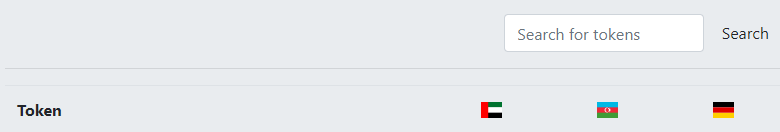
\includegraphics[width=\textwidth]{TR_UI_TOKENS_OLD.png}
    \caption{Ehemalige Tokenübersicht }
  \end{figure}
  \begin{figure}[htb]
    \centering
    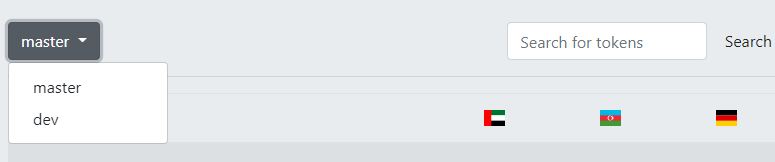
\includegraphics[width=\textwidth]{TR_UI_TOKENS_NEW.png}
    \caption{Neue Tokenübersicht }
  \end{figure}
  \newpage
  \subsection{Aktivitätsdiagramm Translationupdater}\label{sec:activ}
  \begin{figure}[htb]
    \centering
    \includegraphics[width=\textwidth]{Aktivitätsdiagramm_TU.png}
    \caption{Aktivitätsdiagramm Translationupdater}
  \end{figure}
  \newpage
  \subsection{Datenbeschaffung}\label{sec:impl:algo:load}
  \begin{figure}[ht]
    \centering
    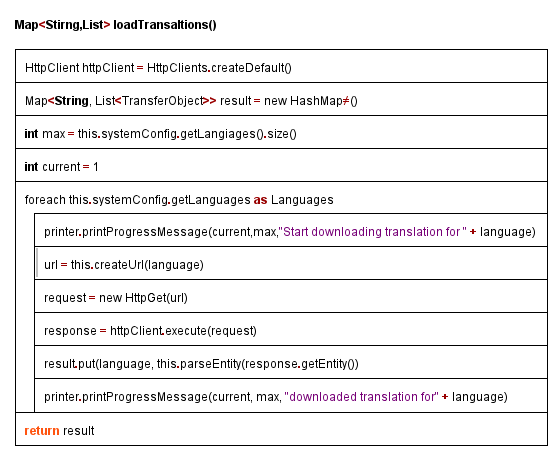
\includegraphics[width=0.9\textwidth]{Beschaffungsalgorithmus.PNG}
    \caption{Nassi-Shneiderman Diagramm Datenbeschaffung}
  \end{figure}
  \newpage
  \section{Listings}
  \subsection{Many-To-Many Annotation}\label{sec:lst:mtmA}
    Token.php
  \begin{lstlisting}[caption={ManyToMany mit Doctrine}, captionpos=b]
    /**
     * @var Version[]|ArrayCollection
     * @ORM\ManyToMany (targetEntity="OktoCareer\TranslationService\
        Version\Version", inversedBy="tokens")
     * @ORM\JoinTable (name="token_version",
     *   joinColumns = {
     *    @ORM\JoinColumn (name="token_id", referencedColumnName="id")
     * },
     *   inverseJoinColumns={
     *    @ORM\JoinColumn (name="version_id", referencedColumnName="id")
     * }
     *     )
     */
     private $version;
  \end{lstlisting}
  Version.php
  \begin{lstlisting}[caption={Many To Many mit Doctrine}, captionpos=b]
    /**
     * @var Token[]|ArrayCollection
     * @ORM\ManyToMany (targetEntity="OktoCareer\TranslationService\
        Token\Token",mappedBy="version")
     */
     private $tokens;
  \end{lstlisting}
  \subsection{Routing}\label{sec:lst:routes}
  HTTP GET Route:
  \begin{lstlisting}[caption={Erstellen einer HTTP GET Route}, captionpos=b, label=lst:impl:bl:GET]
    $app->get('/api/v1/version/{version}/translations/{language}'
      ,ExportTranslationAction::class);
  \end{lstlisting}
  HTTP POST Route:
  \begin{lstlisting}[caption={Erstellen einer HTTP POST Route}, captionpos=b, label=lst:impl:bl:POST]
    $app->post('/api/v1/version/{version}/diff/translations/{language}'
      ,CreateTranslationDiff::class);
  \end{lstlisting}
  \newpage
  \subsection{Configuration.ini}\label{lst:impl:ul:config}
    \begin{lstlisting}[caption={Verwendete Konfigurationsdatei}, captionpos=b]
      [Webservice]
        # Defines the Url to the TranslationService
        baseUrl=http://localhost

        [Cashdesk Properties]
        # Defines the language-files to update
        # e.g fr,en,en-UK,it,sv,es,ja,tr
        languages=de,fr,en

        # Defines the version to download
        version=dev
    \end{lstlisting}
  \subsection{Singleton}\label{sec:lst:singleton}
  \begin{lstlisting}[caption={Singlton in Java}, captionpos=b]
    private static SystemConfig instance;
    private Properties properties;

    private String baseUrl;
    private String languageList;
    private String version;

    public static SystemConfig getInstance() {
        if(instance == null) {
            instance = new SystemConfig();
        }
        return instance;
    }

    private SystemConfig(){
        try {
            loadProperties();
            loadConfiguration();
        } catch (IOException e) {
            System.out.println("Configuration file not found");
        }
    }
  \end{lstlisting}
\end{document}